\documentclass[11pt]{article}
\usepackage[letterpaper,landscape,margin=0.65in]{geometry}
\usepackage{booktabs,graphicx,xcolor}
\setlength{\parindent}{0pt}
\setlength{\parskip}{6pt}
\begin{document}
\begin{center}\Large\textbf{Figure 6 without individual choice-share controls}\end{center}
\textbf{What is plotted.} Average marginal effects from Figure 6's four-category multinomial logit,
re-estimated separately in each subgroup. Both maximum and minimum individual CCEI enter together.
Points measure the probability change, in percentage points, per 0.1 increase in individual CCEI;
bars are 95\% class-clustered confidence intervals. All panels use the same axis, from $-30$ to $50$ points.

\textbf{Main comparison.} The weaker minimum-CCEI association among friendship and higher-math groups
largely carries over to the probability of full group consistency. The wave comparison does not:
the minimum-CCEI marginal effect on reaching group CCEI equal to one is larger at endline.
These endpoint outcomes differ from the continuous group-index regressions previously reported.

\begin{center}\small
\begin{tabular}{lrrrr}\toprule
& \multicolumn{2}{c}{Probability of CCEI $=1$} & \multicolumn{2}{c}{Probability of CEIV $=1$}\\
Split & Lower proxy & Higher proxy & Lower proxy & Higher proxy\\\midrule
Baseline / endline & 3.37 & 5.21 & -0.19 & -0.27\\
No / any friendship nomination & 6.78 & -1.33 & 0.26 & -3.81\\
Pair math: below / at-or-above wave median & 5.90 & 2.82 & 1.70 & -2.66\\
Less-rational math: below / at-or-above wave median & 4.40 & 1.88 & -1.61 & -2.94\\
\bottomrule\end{tabular}\end{center}
\small
The table sums the minimum-CCEI marginal effects across the relevant categories. It reports point estimates,
not formal tests of differences across subgroups. Comparing which confidence intervals contain zero is not a test
of heterogeneity. Subgroup distributions and room for improvement also differ.

\textbf{Same controls as Figure 6.} Student/personality and friendship/network controls,
plus class fixed effects and class-clustered standard errors. Individual corner- and midpoint-choice shares are excluded. No risk-aversion controls or risk-gap restriction.
The primary non-wave splits pool baseline and endline, as in the preceding heterogeneity analysis.
CCEI and CEIV equal one when their computed value is at least $1-10^{-9}$; CEIV lower and upper bounds agree
on this classification. All successful separate fits retain their entire eligible subgroup.

\textbf{Small-subgroup limitation.} The mutual-friendship sample has 167 observations and 54 classes.
Its separate model does not produce a converged, validated fit with either omitted-outcome parameterization.
The final page therefore shows an explicitly labelled alternative: estimate all friendship categories jointly,
interacting both CCEIs with friendship, while sharing the other controls and class effects.

\textbf{Interpretation.} The splits are descriptive communication proxies. Group CCEI measures internal
consistency; it does not identify constant aggregation weights. CEIV does not identify turn-taking.
Experience, friendship, and math scores do not directly measure the content of communication.
\clearpage
\begin{center}\Large\textbf{Does removing choice-share controls change the continuous results?}\end{center}
\textbf{Finding.} The principal minimum-CCEI pattern is essentially unchanged. In the pooled sample its
group-CCEI coefficient moves from 0.235 to 0.228, and its CEIV coefficient from 0.086 to 0.081.
The friendship difference remains clear; wave and math differences remain imprecise.

\begin{center}\small\begin{tabular}{lrrrr}\toprule
& \multicolumn{2}{c}{Group CCEI: minimum individual CCEI} & \multicolumn{2}{c}{CEIV: minimum individual CCEI}\\
Sample & With shares & Without shares & With shares & Without shares\\\midrule
All pair-waves & 0.235 (0.045) & 0.228 (0.044) & 0.086 (0.035) & 0.081 (0.034)\\
Baseline & 0.269 (0.059) & 0.263 (0.060) & 0.077 (0.046) & 0.070 (0.045)\\
Endline & 0.207 (0.060) & 0.194 (0.059) & 0.099 (0.049) & 0.093 (0.049)\\
No friendship nomination & 0.311 (0.050) & 0.299 (0.049) & 0.120 (0.040) & 0.116 (0.040)\\
Any friendship nomination & -0.010 (0.049) & -0.005 (0.049) & -0.056 (0.058) & -0.054 (0.058)\\
Pair math: below median & 0.294 (0.071) & 0.286 (0.069) & 0.131 (0.057) & 0.122 (0.055)\\
Pair math: at/above median & 0.168 (0.058) & 0.160 (0.057) & 0.033 (0.046) & 0.029 (0.047)\\
Less-rational math: below median & 0.285 (0.069) & 0.268 (0.068) & 0.099 (0.056) & 0.092 (0.057)\\
Less-rational math: at/above median & 0.176 (0.061) & 0.161 (0.060) & 0.045 (0.047) & 0.036 (0.047)\\
\bottomrule\end{tabular}\end{center}
\small
Coefficients are per one-unit increase in individual CCEI, with class-clustered standard errors in parentheses.
Multiply by 0.1 for a 0.1 increase. Both individual CCEIs enter together. The original and reduced-control models
use identical samples and retain class fixed effects and all other controls. These continuous regressions differ
from the four-category multinomial probability model shown in the remaining figures.

\textbf{Formal differences without choice-share controls.} Any friendship nomination minus none changes the
minimum-CCEI slope by $-0.304$ for group CCEI ($p<0.001$), and $-0.170$ for CEIV ($p=0.023$).
The larger decline for group CCEI is supported by the direct cross-outcome test ($p=0.005$).
The group-CCEI slope differences have $p=0.390$ for endline minus baseline, $p=0.169$ for higher minus lower
pair math, and $p=0.200$ for higher minus lower less-rational-member math.

\textbf{What this check addresses.} Individual CCEI and these choice shares are calculated from the same individual
choices. Including the shares asks about rationality conditional on those choice patterns; excluding them gives a
broader adjusted association. The similarity of results reduces concern that those controls drive the present pattern.
It does not identify the bargaining or communication process.
\clearpage
\begin{center}\Large\textbf{Baseline}\end{center}
\small The same 652 pairs are observed in each wave. Endline may capture experience as well as other changes between waves.
Separate-subgroup fit: 652 pair-waves, 652 distinct pairs, 64 class clusters.
\begin{center}\begin{minipage}{0.48\textwidth}\centering
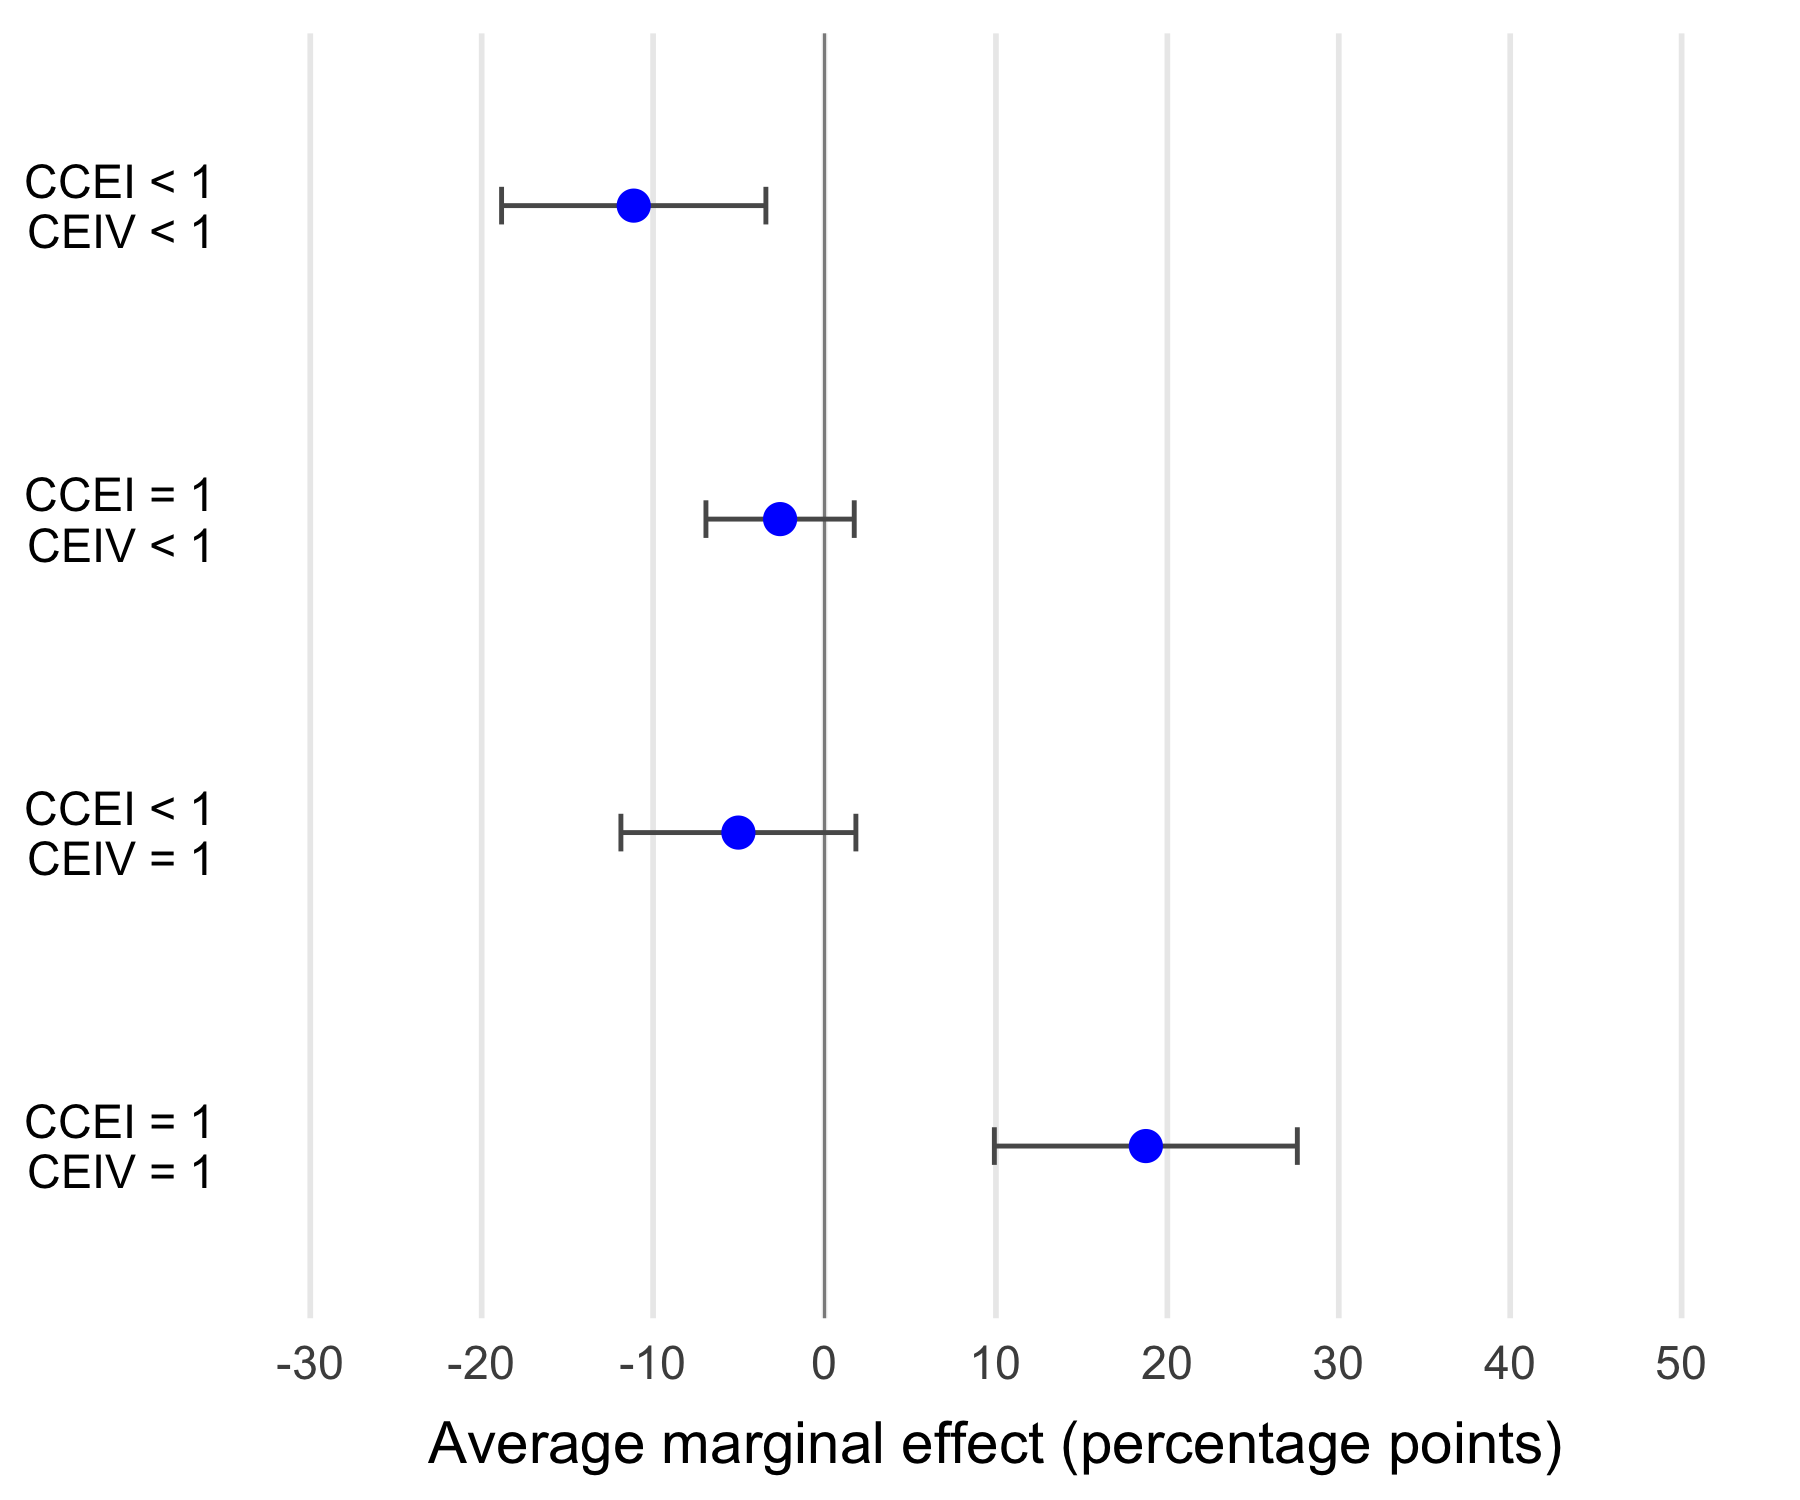
\includegraphics[width=\linewidth]{figure6_a_wave_0_ame_maximum.png}
\textbf{(a) More rational member: maximum CCEI}\end{minipage}\hfill\begin{minipage}{0.48\textwidth}\centering
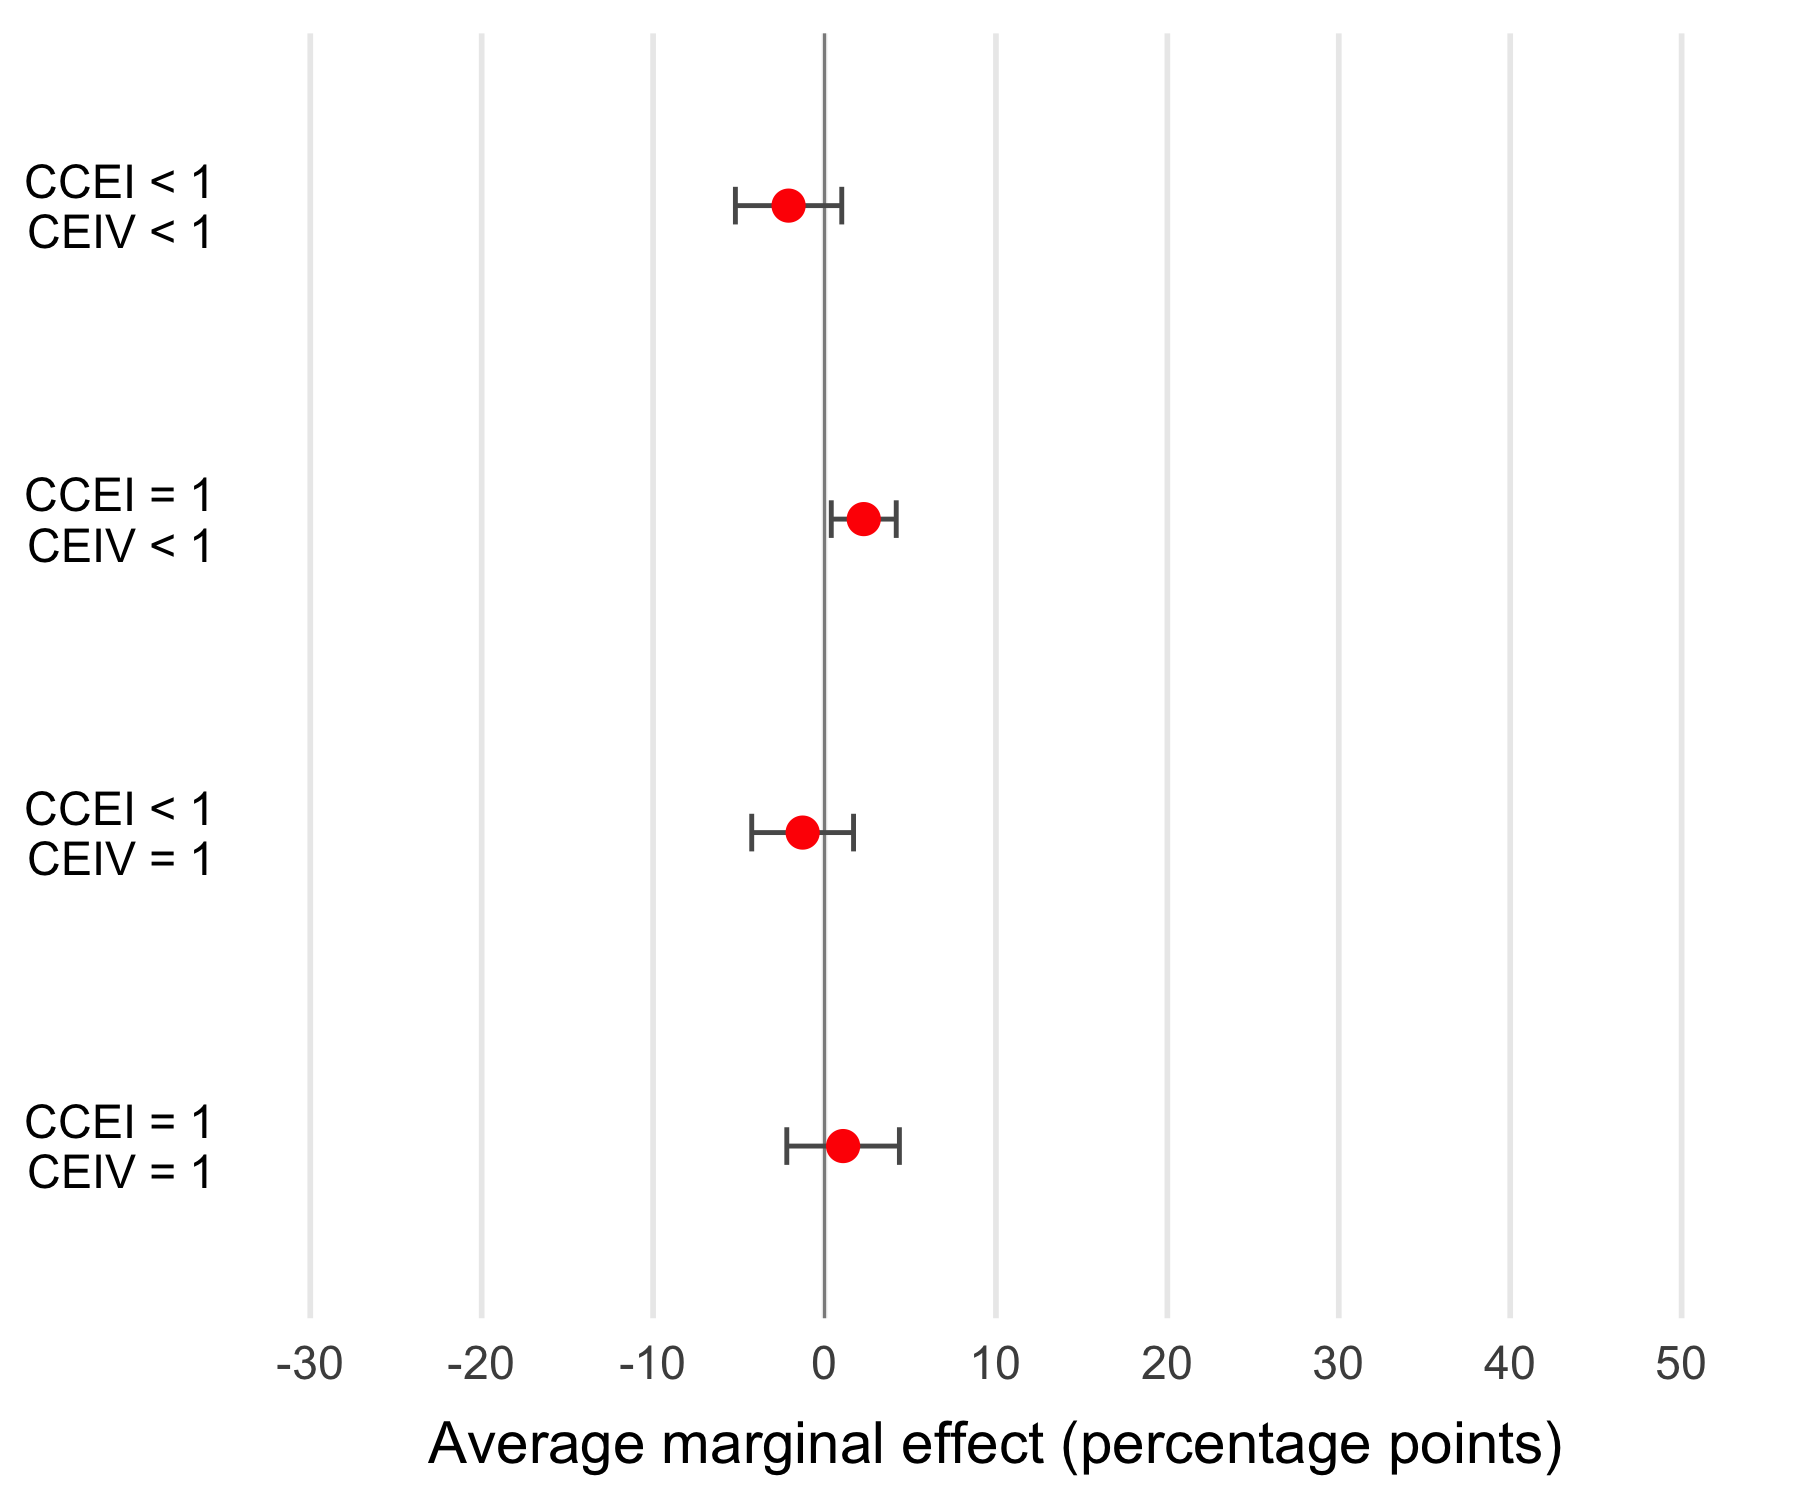
\includegraphics[width=\linewidth]{figure6_a_wave_0_ame_minimum.png}
\textbf{(b) Less rational member: minimum CCEI}\end{minipage}\end{center}
\begin{center}\begin{tabular}{lrrrr}\toprule
Outcome & CCEI $<1$, CEIV $<1$ & CCEI $=1$, CEIV $<1$ & CCEI $<1$, CEIV $=1$ & CCEI $=1$, CEIV $=1$\\\midrule
Observed pair-waves & 232 & 67 & 165 & 188\\
Share & 35.6\% & 10.3\% & 25.3\% & 28.8\%\\\bottomrule\end{tabular}\end{center}
\footnotesize\textit{Notes:} Effects are percentage points per 0.1 increase in individual CCEI, holding the other member's CCEI and controls fixed locally, then averaging over this subgroup. Four-category effects sum to zero for each member. Intervals use class-clustered standard errors. The class effects, coefficients, and outcome distributions can differ across separate fits; visual comparisons are descriptive.
\clearpage
\begin{center}\Large\textbf{Endline}\end{center}
\small The same 652 pairs are observed in each wave. Endline may capture experience as well as other changes between waves.
Separate-subgroup fit: 652 pair-waves, 652 distinct pairs, 64 class clusters.
\begin{center}\begin{minipage}{0.48\textwidth}\centering
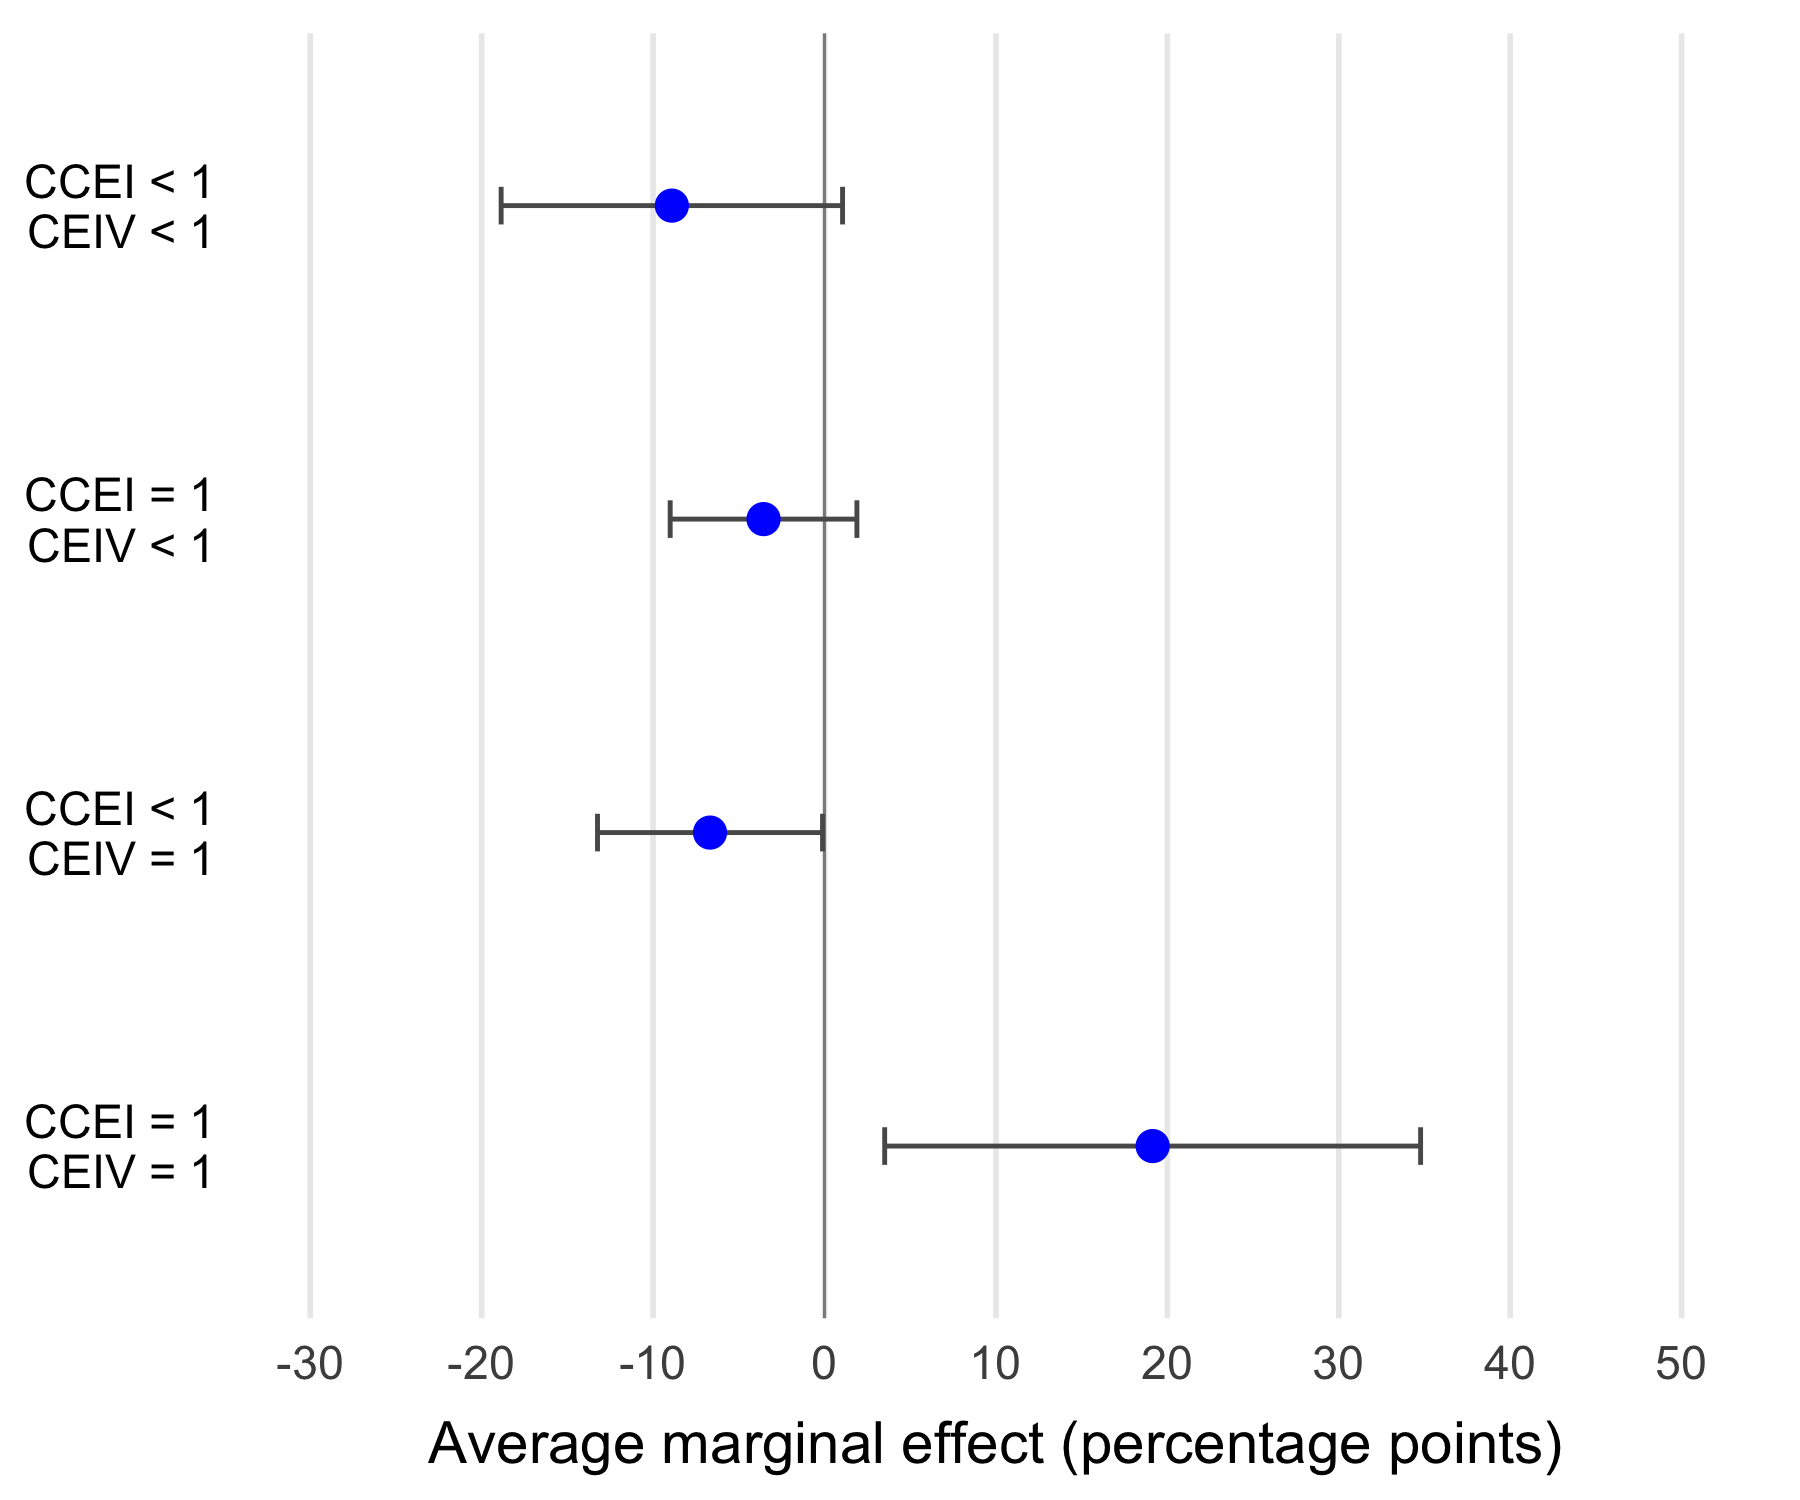
\includegraphics[width=\linewidth]{figure6_a_wave_1_ame_maximum.png}
\textbf{(a) More rational member: maximum CCEI}\end{minipage}\hfill\begin{minipage}{0.48\textwidth}\centering
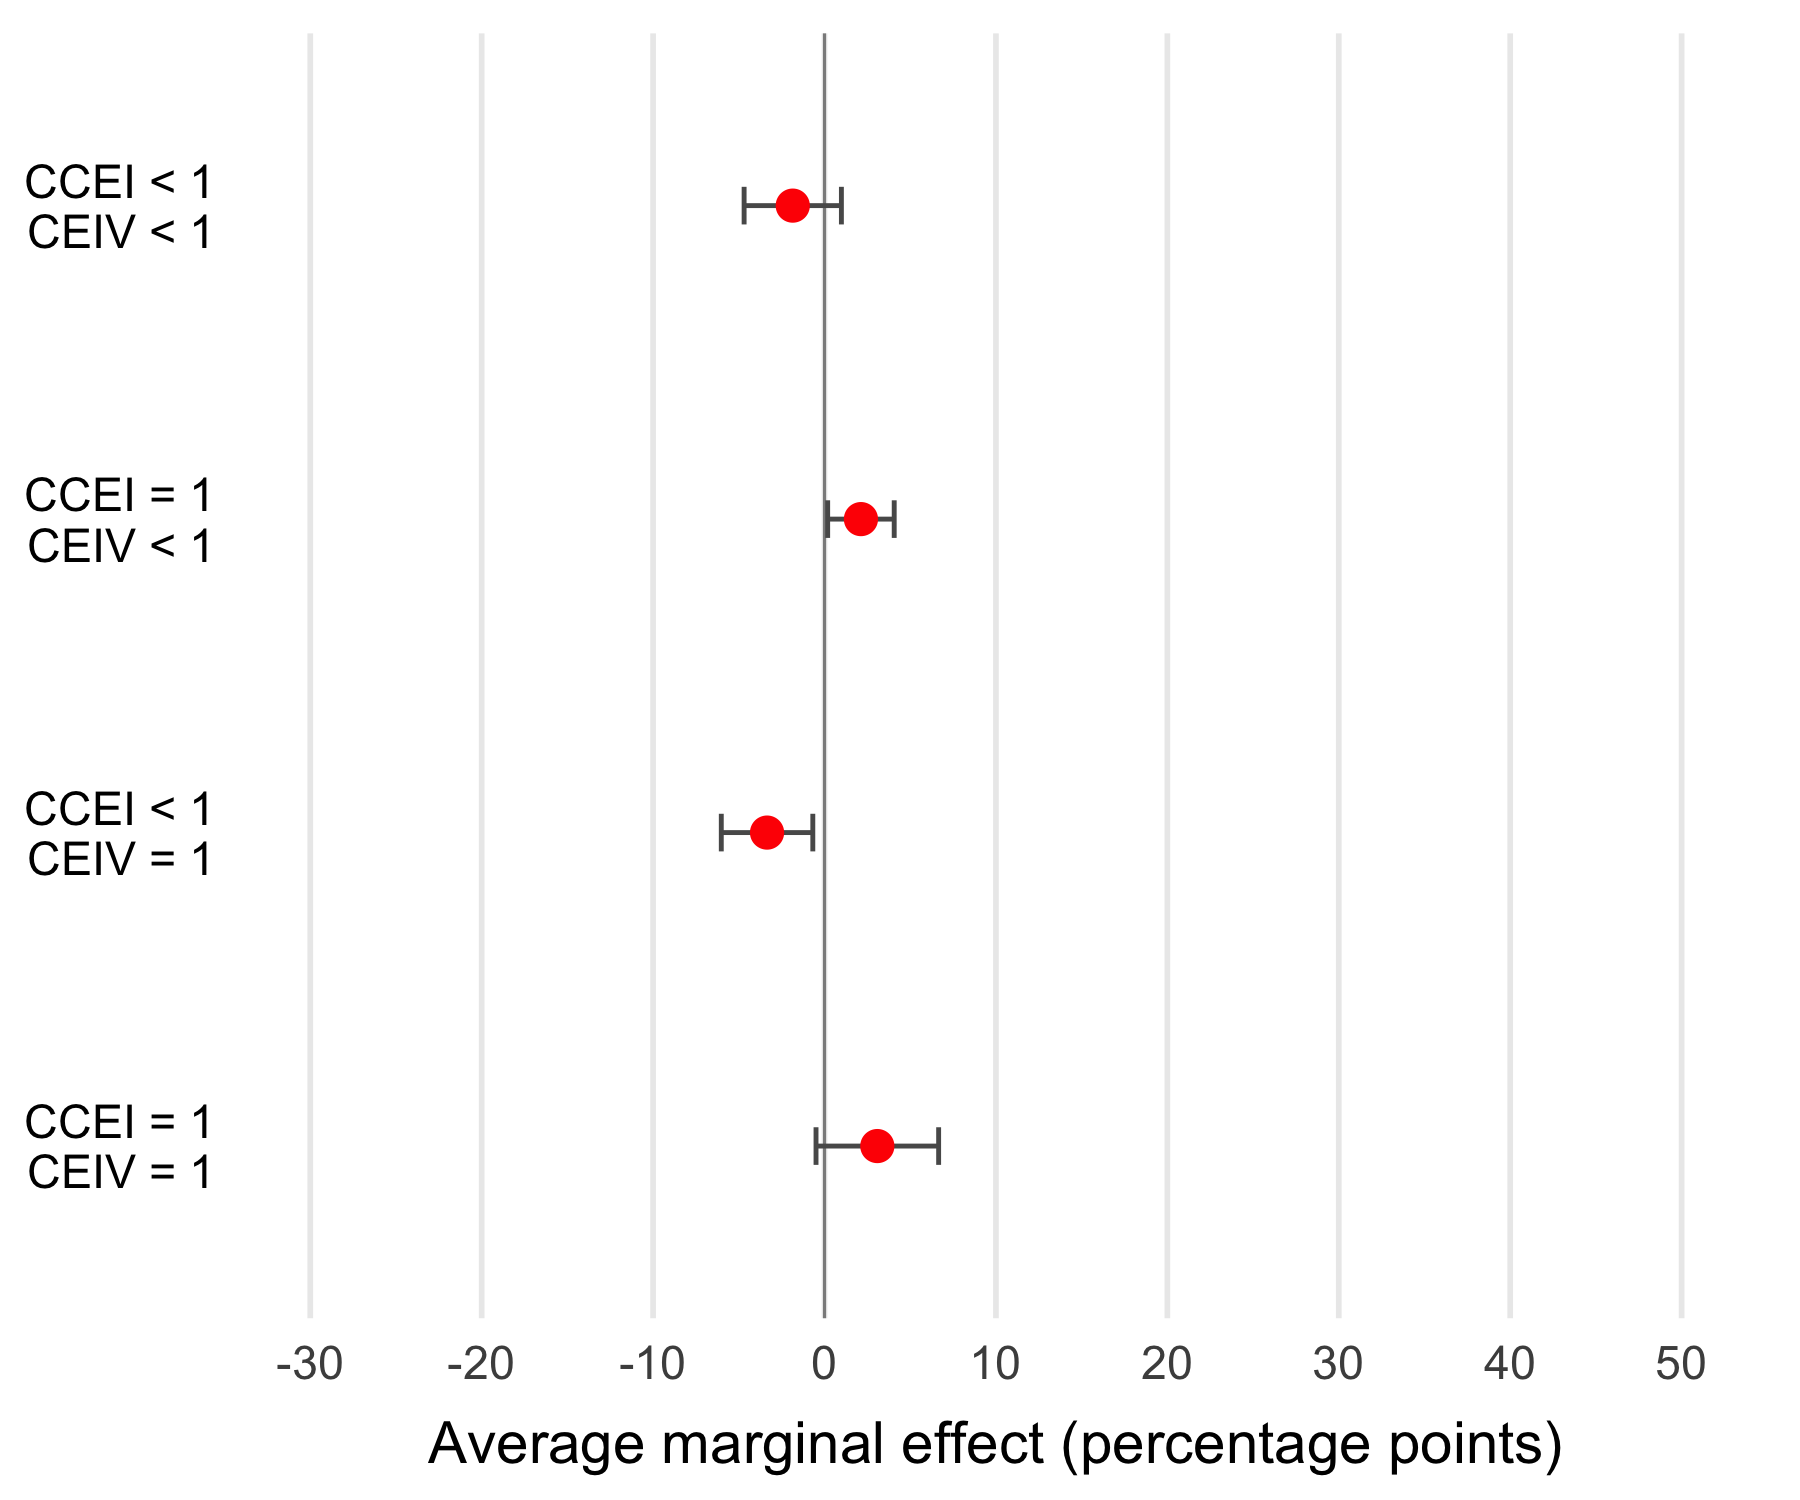
\includegraphics[width=\linewidth]{figure6_a_wave_1_ame_minimum.png}
\textbf{(b) Less rational member: minimum CCEI}\end{minipage}\end{center}
\begin{center}\begin{tabular}{lrrrr}\toprule
Outcome & CCEI $<1$, CEIV $<1$ & CCEI $=1$, CEIV $<1$ & CCEI $<1$, CEIV $=1$ & CCEI $=1$, CEIV $=1$\\\midrule
Observed pair-waves & 183 & 50 & 135 & 284\\
Share & 28.1\% & 7.7\% & 20.7\% & 43.6\%\\\bottomrule\end{tabular}\end{center}
\footnotesize\textit{Notes:} Effects are percentage points per 0.1 increase in individual CCEI, holding the other member's CCEI and controls fixed locally, then averaging over this subgroup. Four-category effects sum to zero for each member. Intervals use class-clustered standard errors. The class effects, coefficients, and outcome distributions can differ across separate fits; visual comparisons are descriptive.
\clearpage
\begin{center}\Large\textbf{No friendship nomination}\end{center}
\small Friendship means at least one directed nomination. It is contemporaneous: 167 pairs change the three-category friendship classification between waves.
Separate-subgroup fit: 912 pair-waves, 518 distinct pairs, 64 class clusters.
\begin{center}\begin{minipage}{0.48\textwidth}\centering
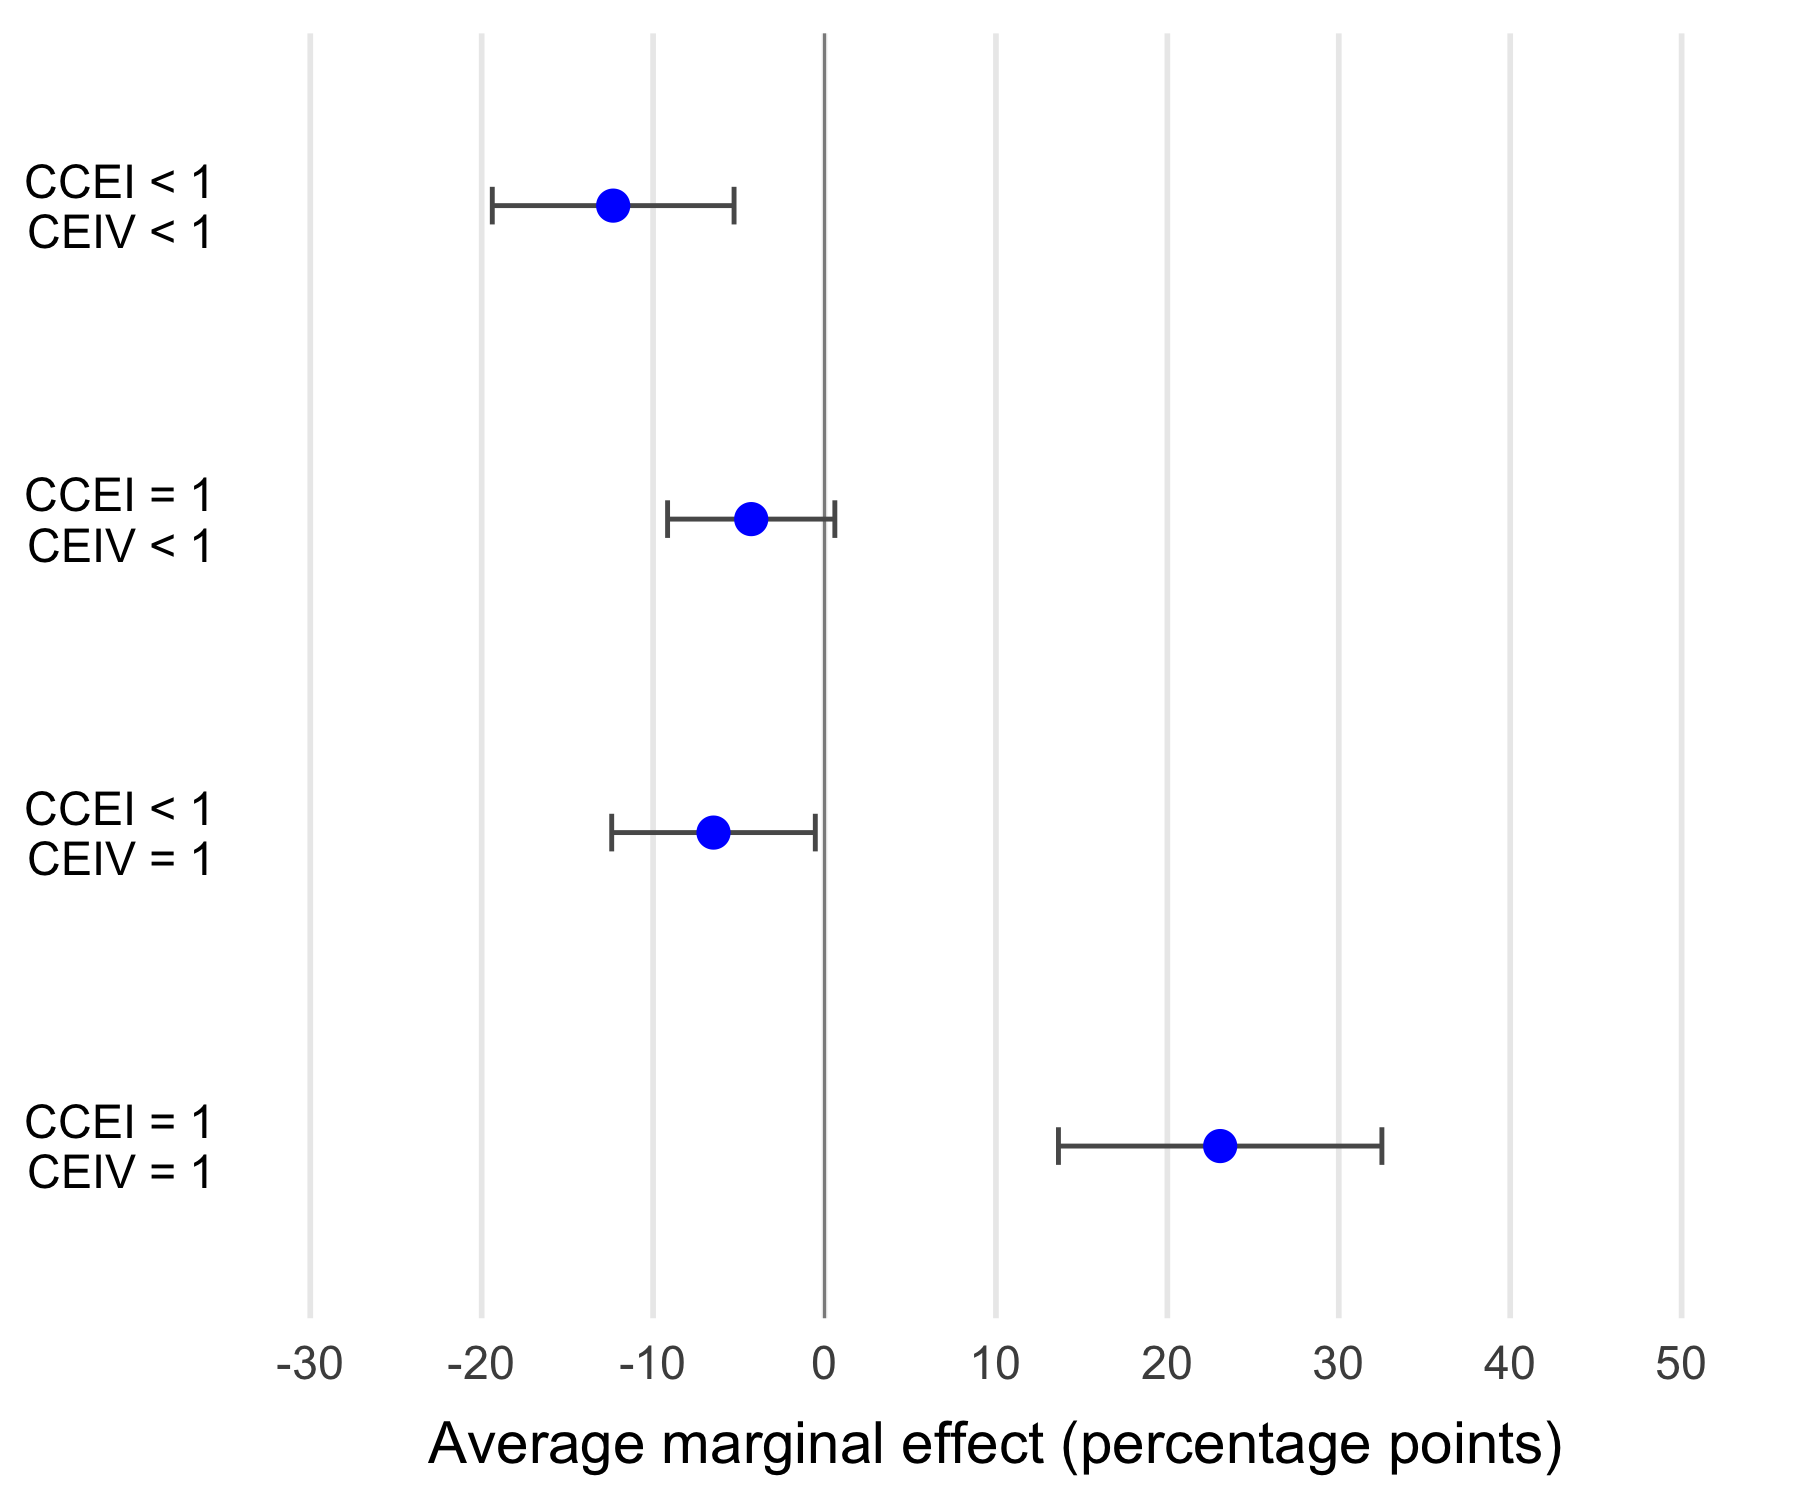
\includegraphics[width=\linewidth]{figure6_a_friend_any_0_ame_maximum.png}
\textbf{(a) More rational member: maximum CCEI}\end{minipage}\hfill\begin{minipage}{0.48\textwidth}\centering
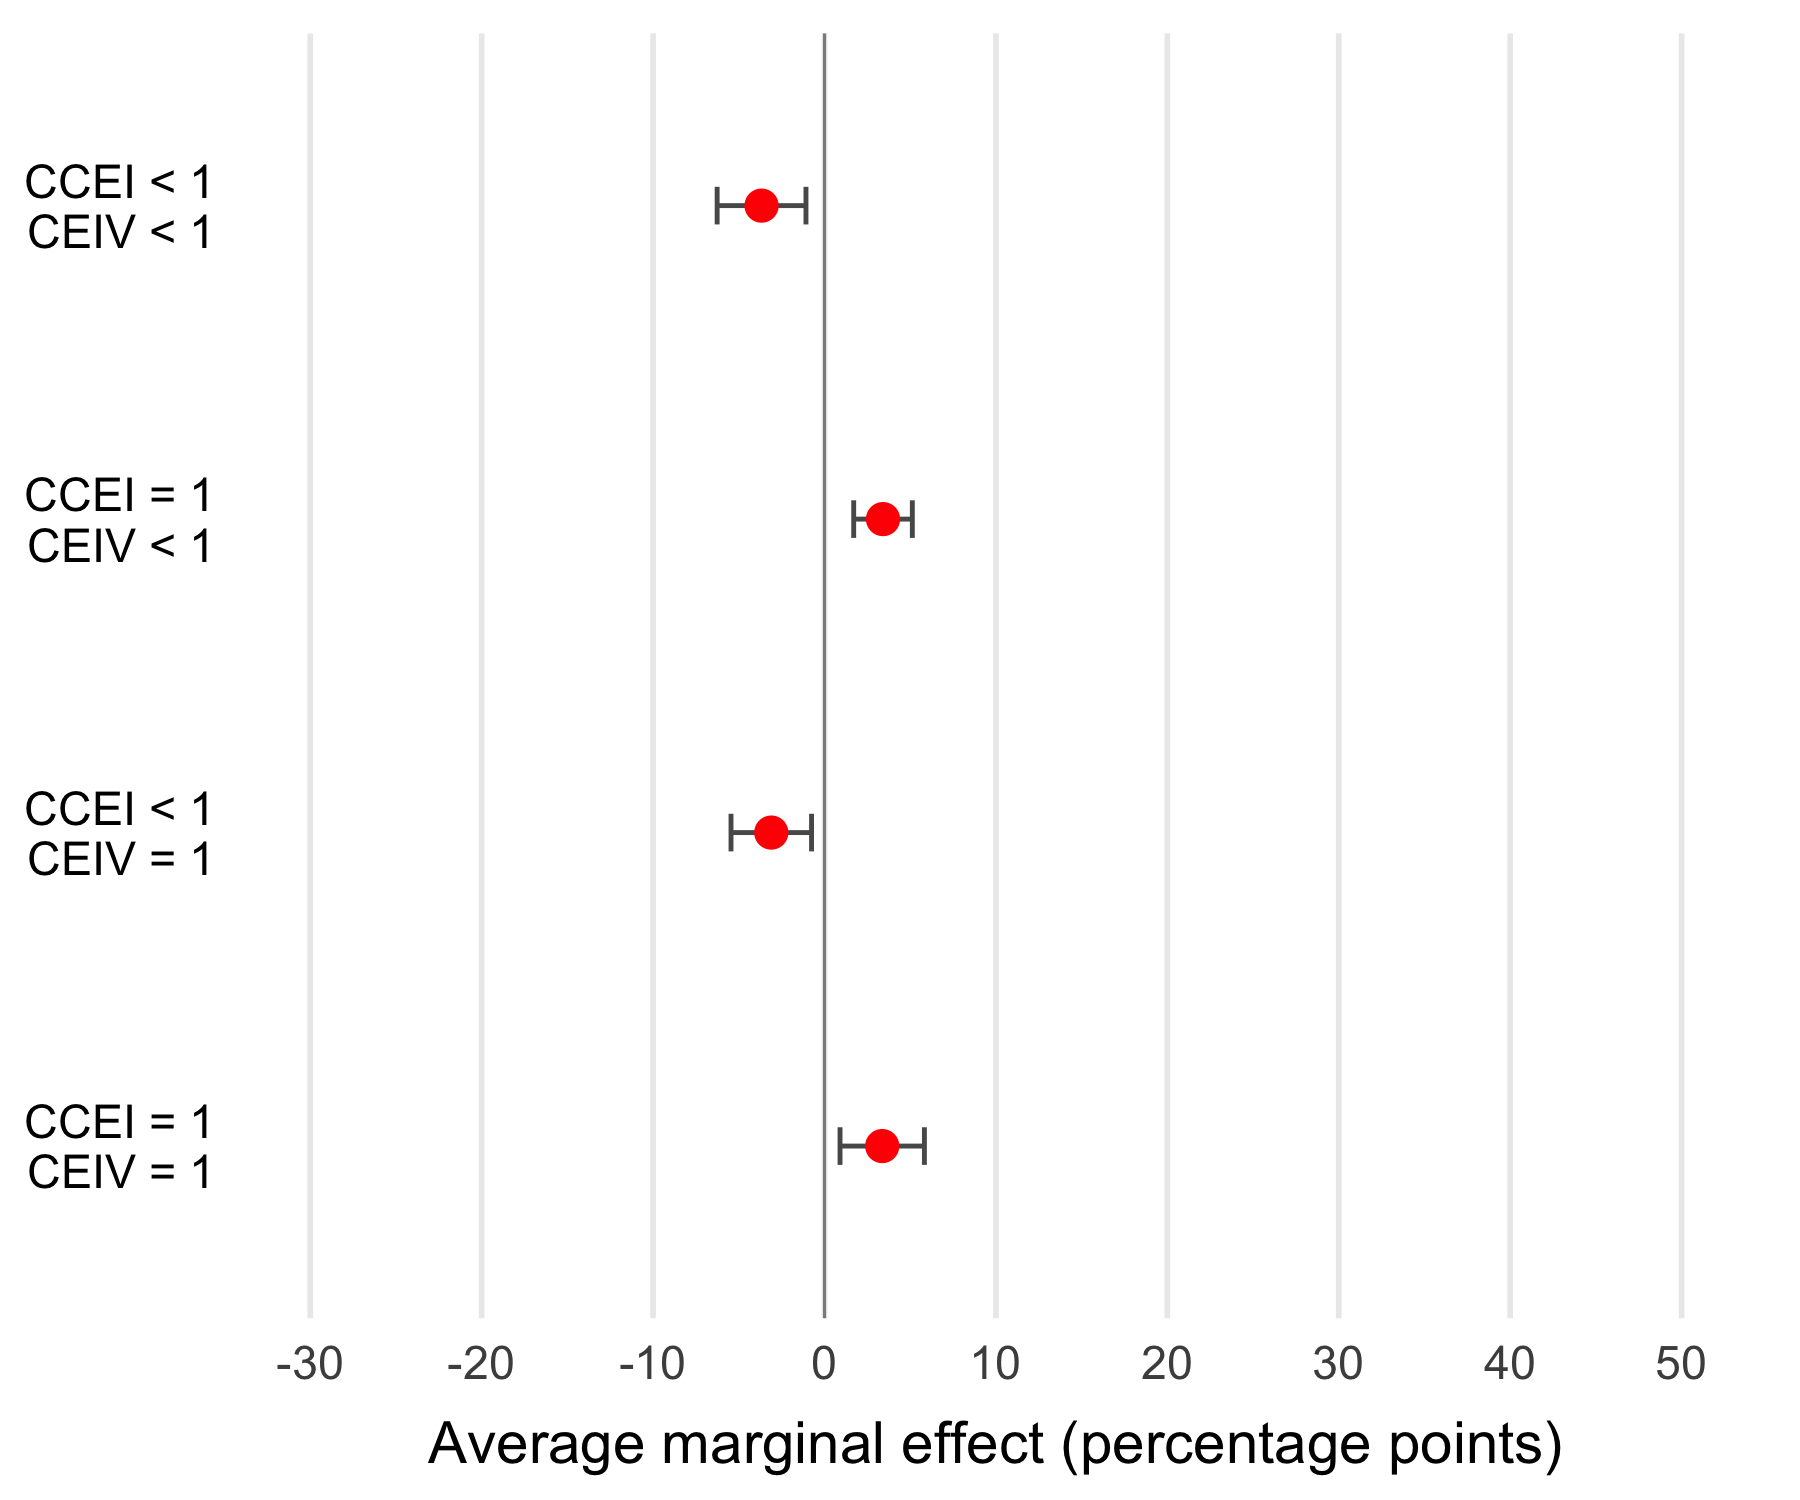
\includegraphics[width=\linewidth]{figure6_a_friend_any_0_ame_minimum.png}
\textbf{(b) Less rational member: minimum CCEI}\end{minipage}\end{center}
\begin{center}\begin{tabular}{lrrrr}\toprule
Outcome & CCEI $<1$, CEIV $<1$ & CCEI $=1$, CEIV $<1$ & CCEI $<1$, CEIV $=1$ & CCEI $=1$, CEIV $=1$\\\midrule
Observed pair-waves & 306 & 80 & 206 & 320\\
Share & 33.6\% & 8.8\% & 22.6\% & 35.1\%\\\bottomrule\end{tabular}\end{center}
\footnotesize\textit{Notes:} Effects are percentage points per 0.1 increase in individual CCEI, holding the other member's CCEI and controls fixed locally, then averaging over this subgroup. Four-category effects sum to zero for each member. Intervals use class-clustered standard errors. The class effects, coefficients, and outcome distributions can differ across separate fits; visual comparisons are descriptive.
\clearpage
\begin{center}\Large\textbf{At least one friendship nomination}\end{center}
\small Friendship means at least one directed nomination. It is contemporaneous: 167 pairs change the three-category friendship classification between waves.
Separate-subgroup fit: 392 pair-waves, 258 distinct pairs, 62 class clusters.
\begin{center}\begin{minipage}{0.48\textwidth}\centering
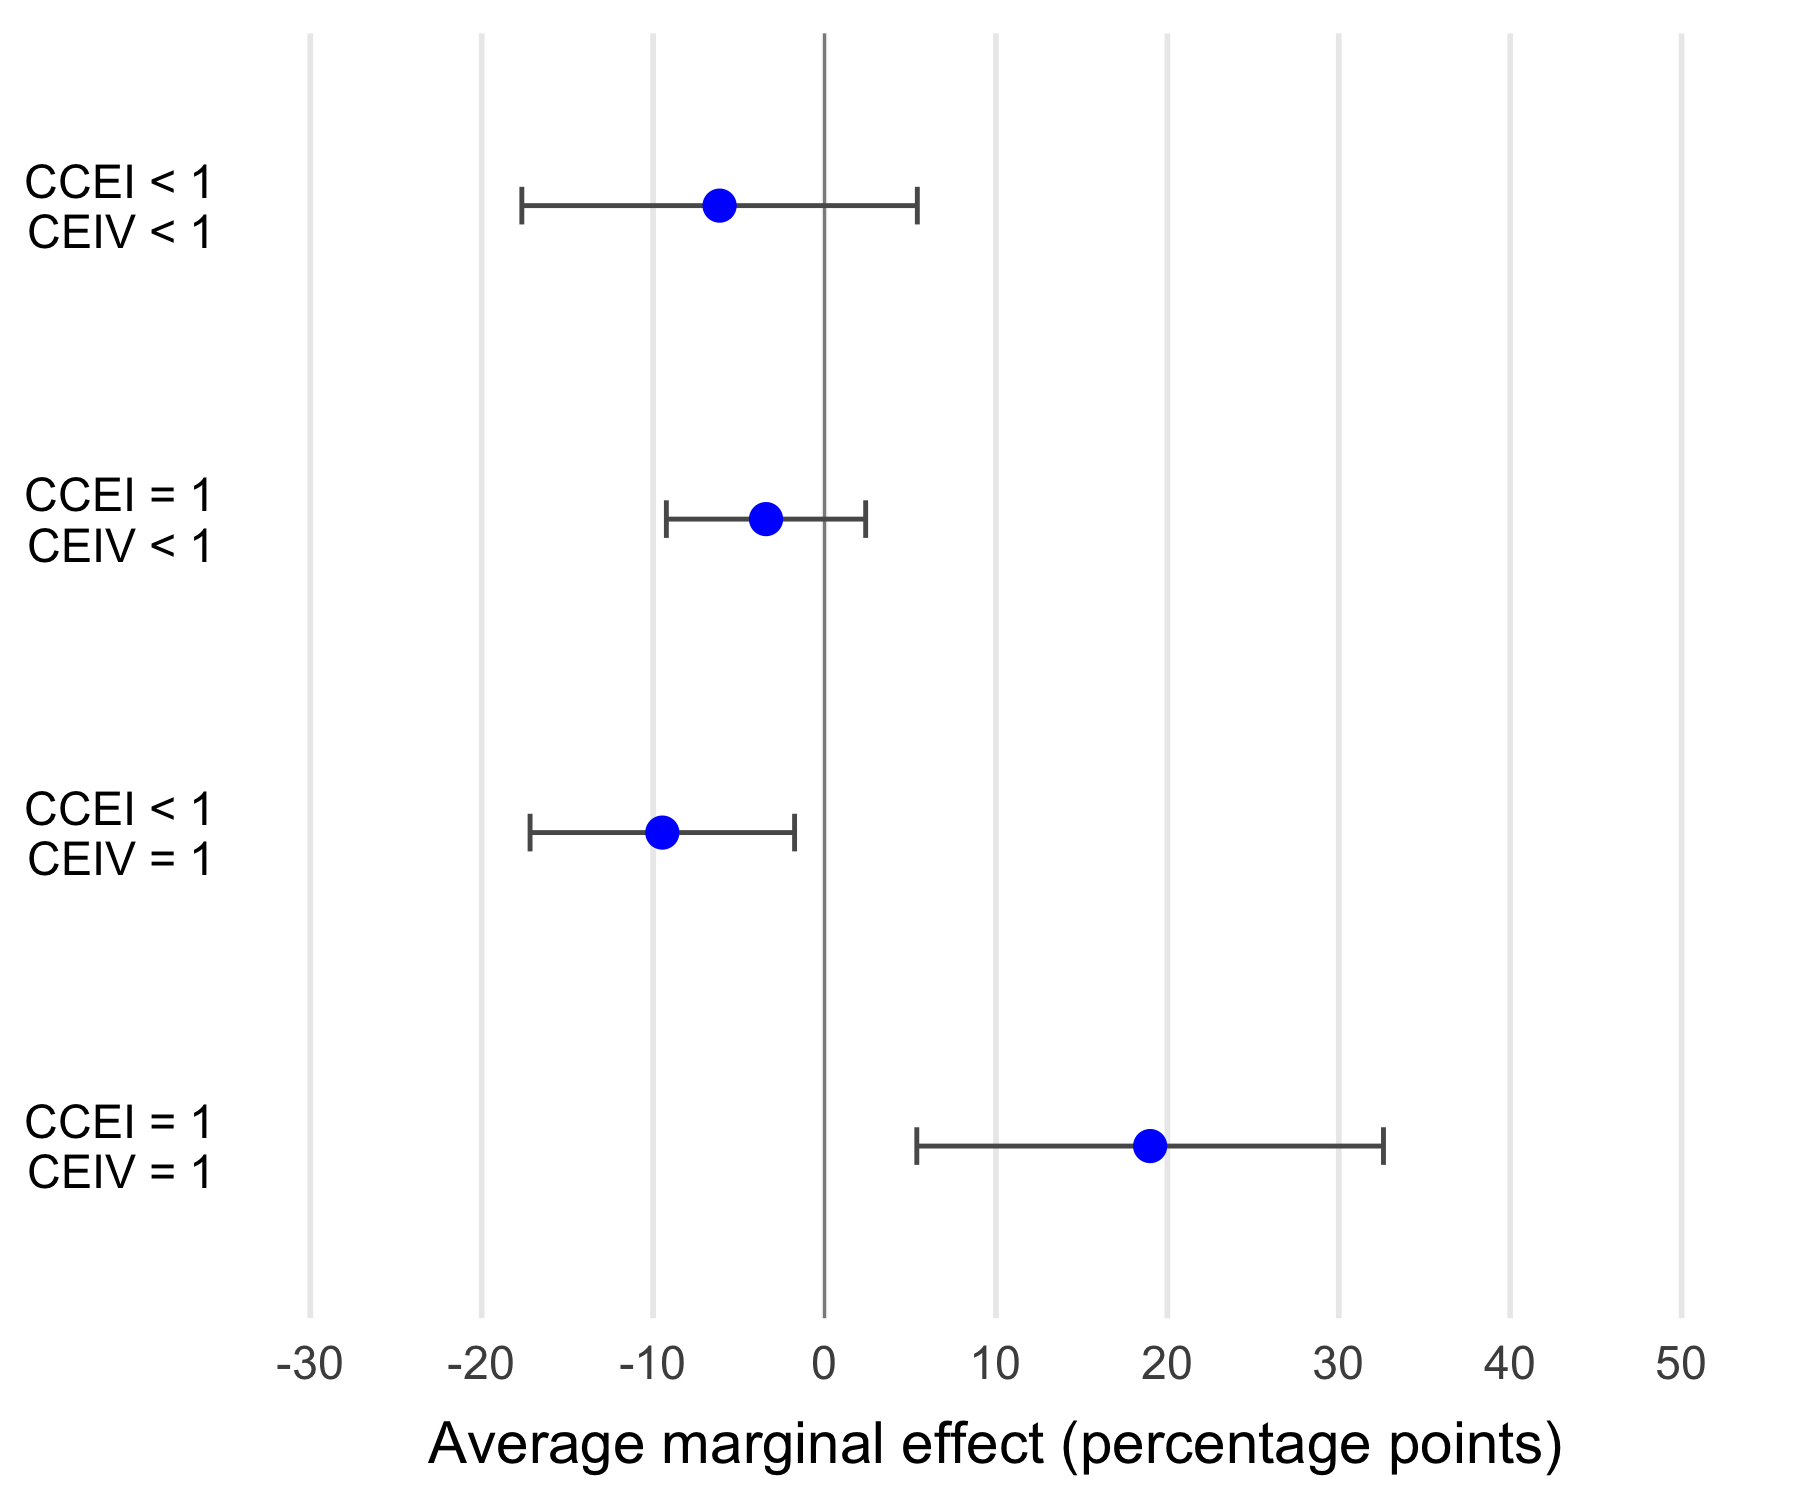
\includegraphics[width=\linewidth]{figure6_a_friend_any_1_ame_maximum.png}
\textbf{(a) More rational member: maximum CCEI}\end{minipage}\hfill\begin{minipage}{0.48\textwidth}\centering
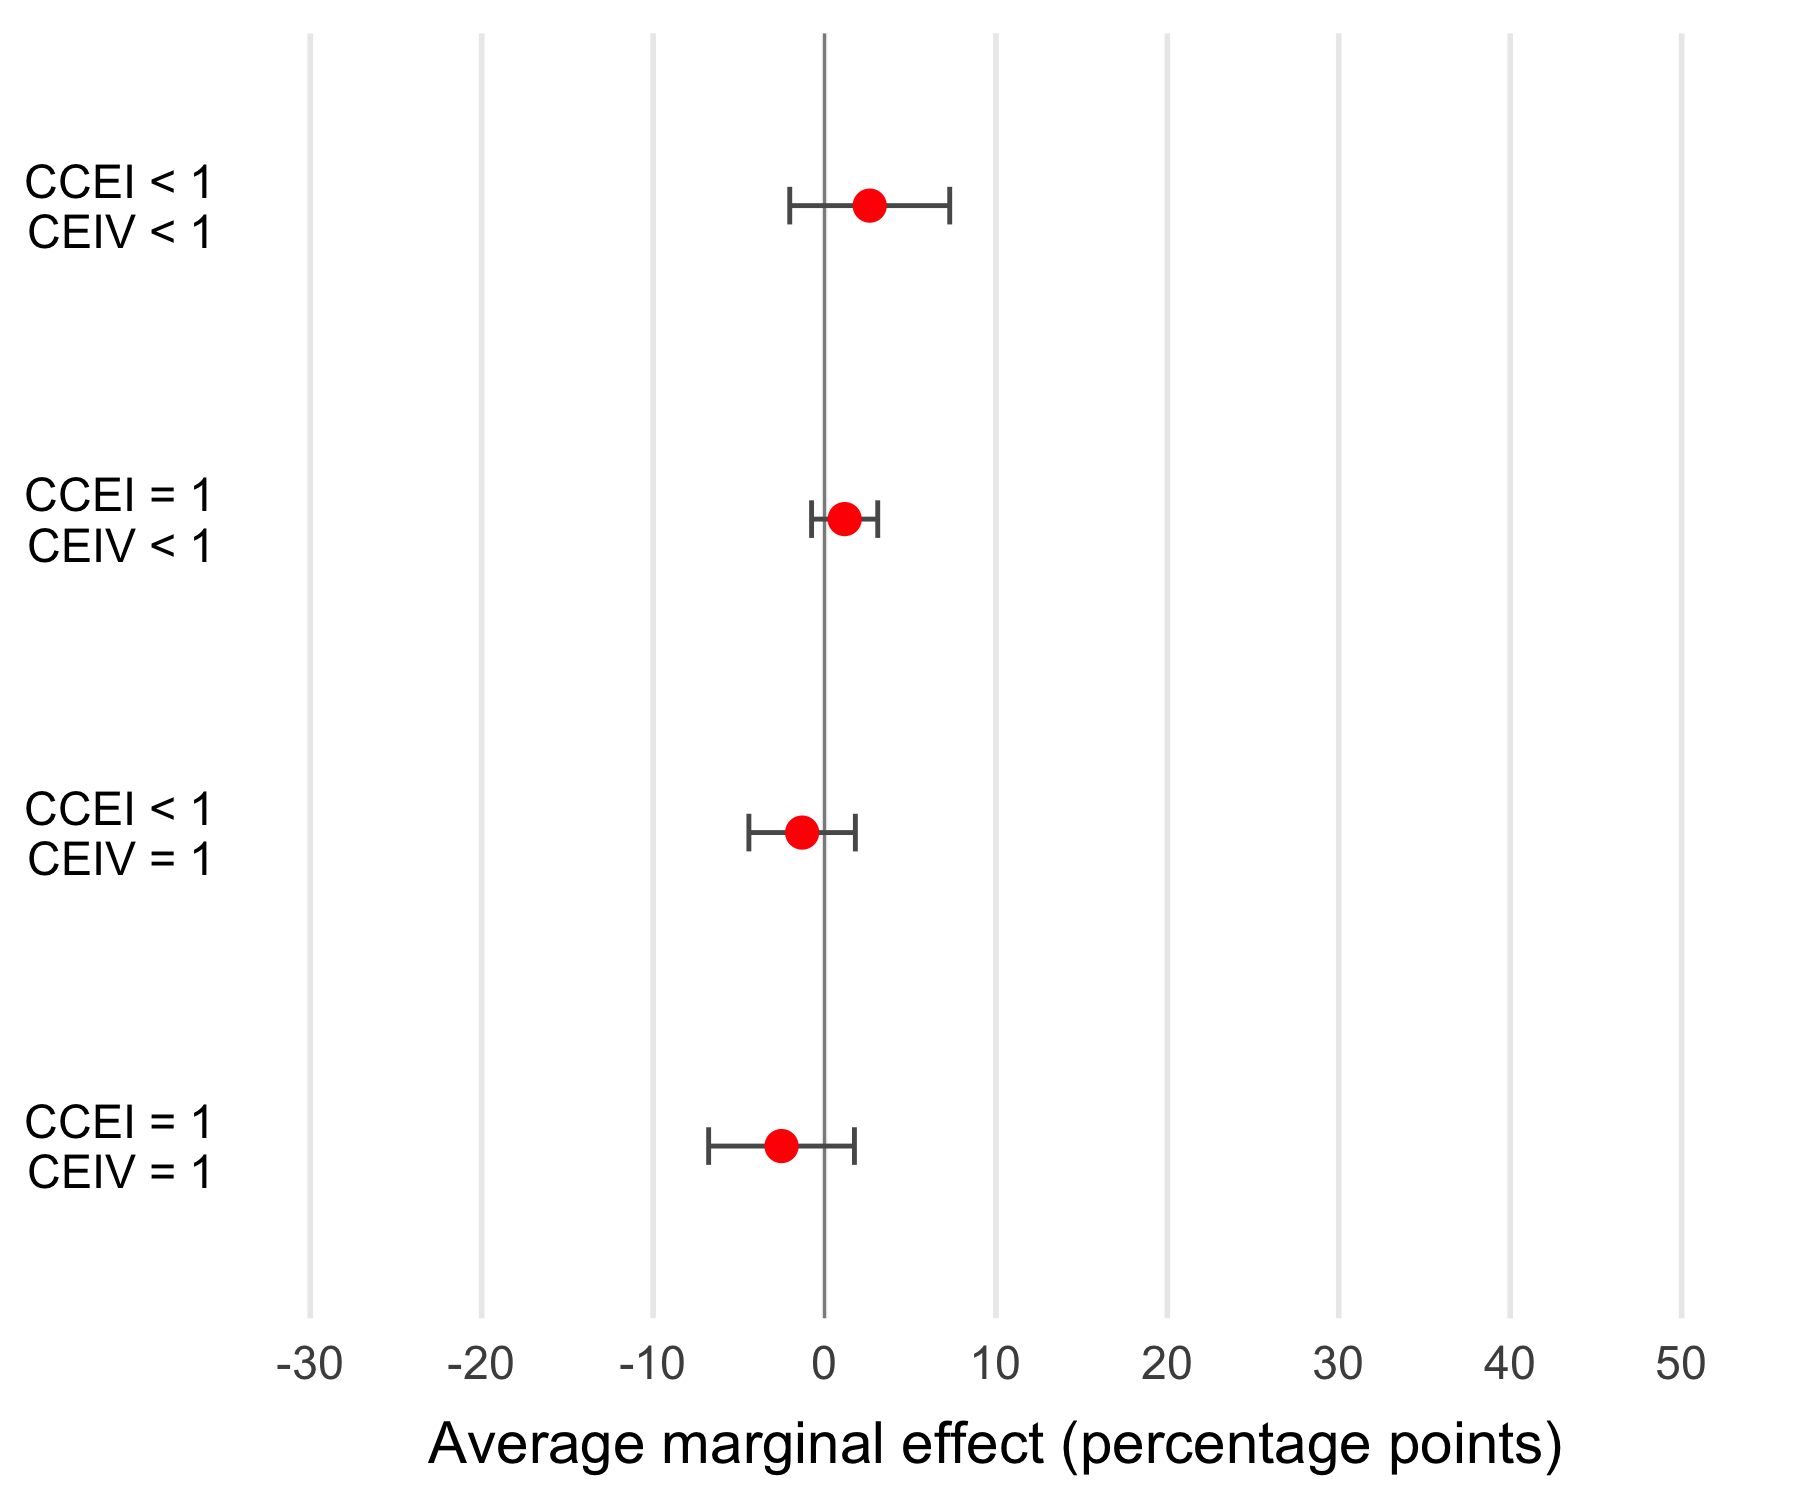
\includegraphics[width=\linewidth]{figure6_a_friend_any_1_ame_minimum.png}
\textbf{(b) Less rational member: minimum CCEI}\end{minipage}\end{center}
\begin{center}\begin{tabular}{lrrrr}\toprule
Outcome & CCEI $<1$, CEIV $<1$ & CCEI $=1$, CEIV $<1$ & CCEI $<1$, CEIV $=1$ & CCEI $=1$, CEIV $=1$\\\midrule
Observed pair-waves & 109 & 37 & 94 & 152\\
Share & 27.8\% & 9.4\% & 24.0\% & 38.8\%\\\bottomrule\end{tabular}\end{center}
\footnotesize\textit{Notes:} Effects are percentage points per 0.1 increase in individual CCEI, holding the other member's CCEI and controls fixed locally, then averaging over this subgroup. Four-category effects sum to zero for each member. Intervals use class-clustered standard errors. The class effects, coefficients, and outcome distributions can differ across separate fits; visual comparisons are descriptive.
\clearpage
\begin{center}\Large\textbf{Pair-average math: below wave median}\end{center}
\small Average both observed math scores (0--5); exclude 13 pair-waves with a missing score. Wave medians are 2.5 at baseline and 3 at endline. Median ties enter the higher bin; eligible low/high counts are 530/761.
Separate-subgroup fit: 530 pair-waves, 369 distinct pairs, 62 class clusters.
\begin{center}\begin{minipage}{0.48\textwidth}\centering
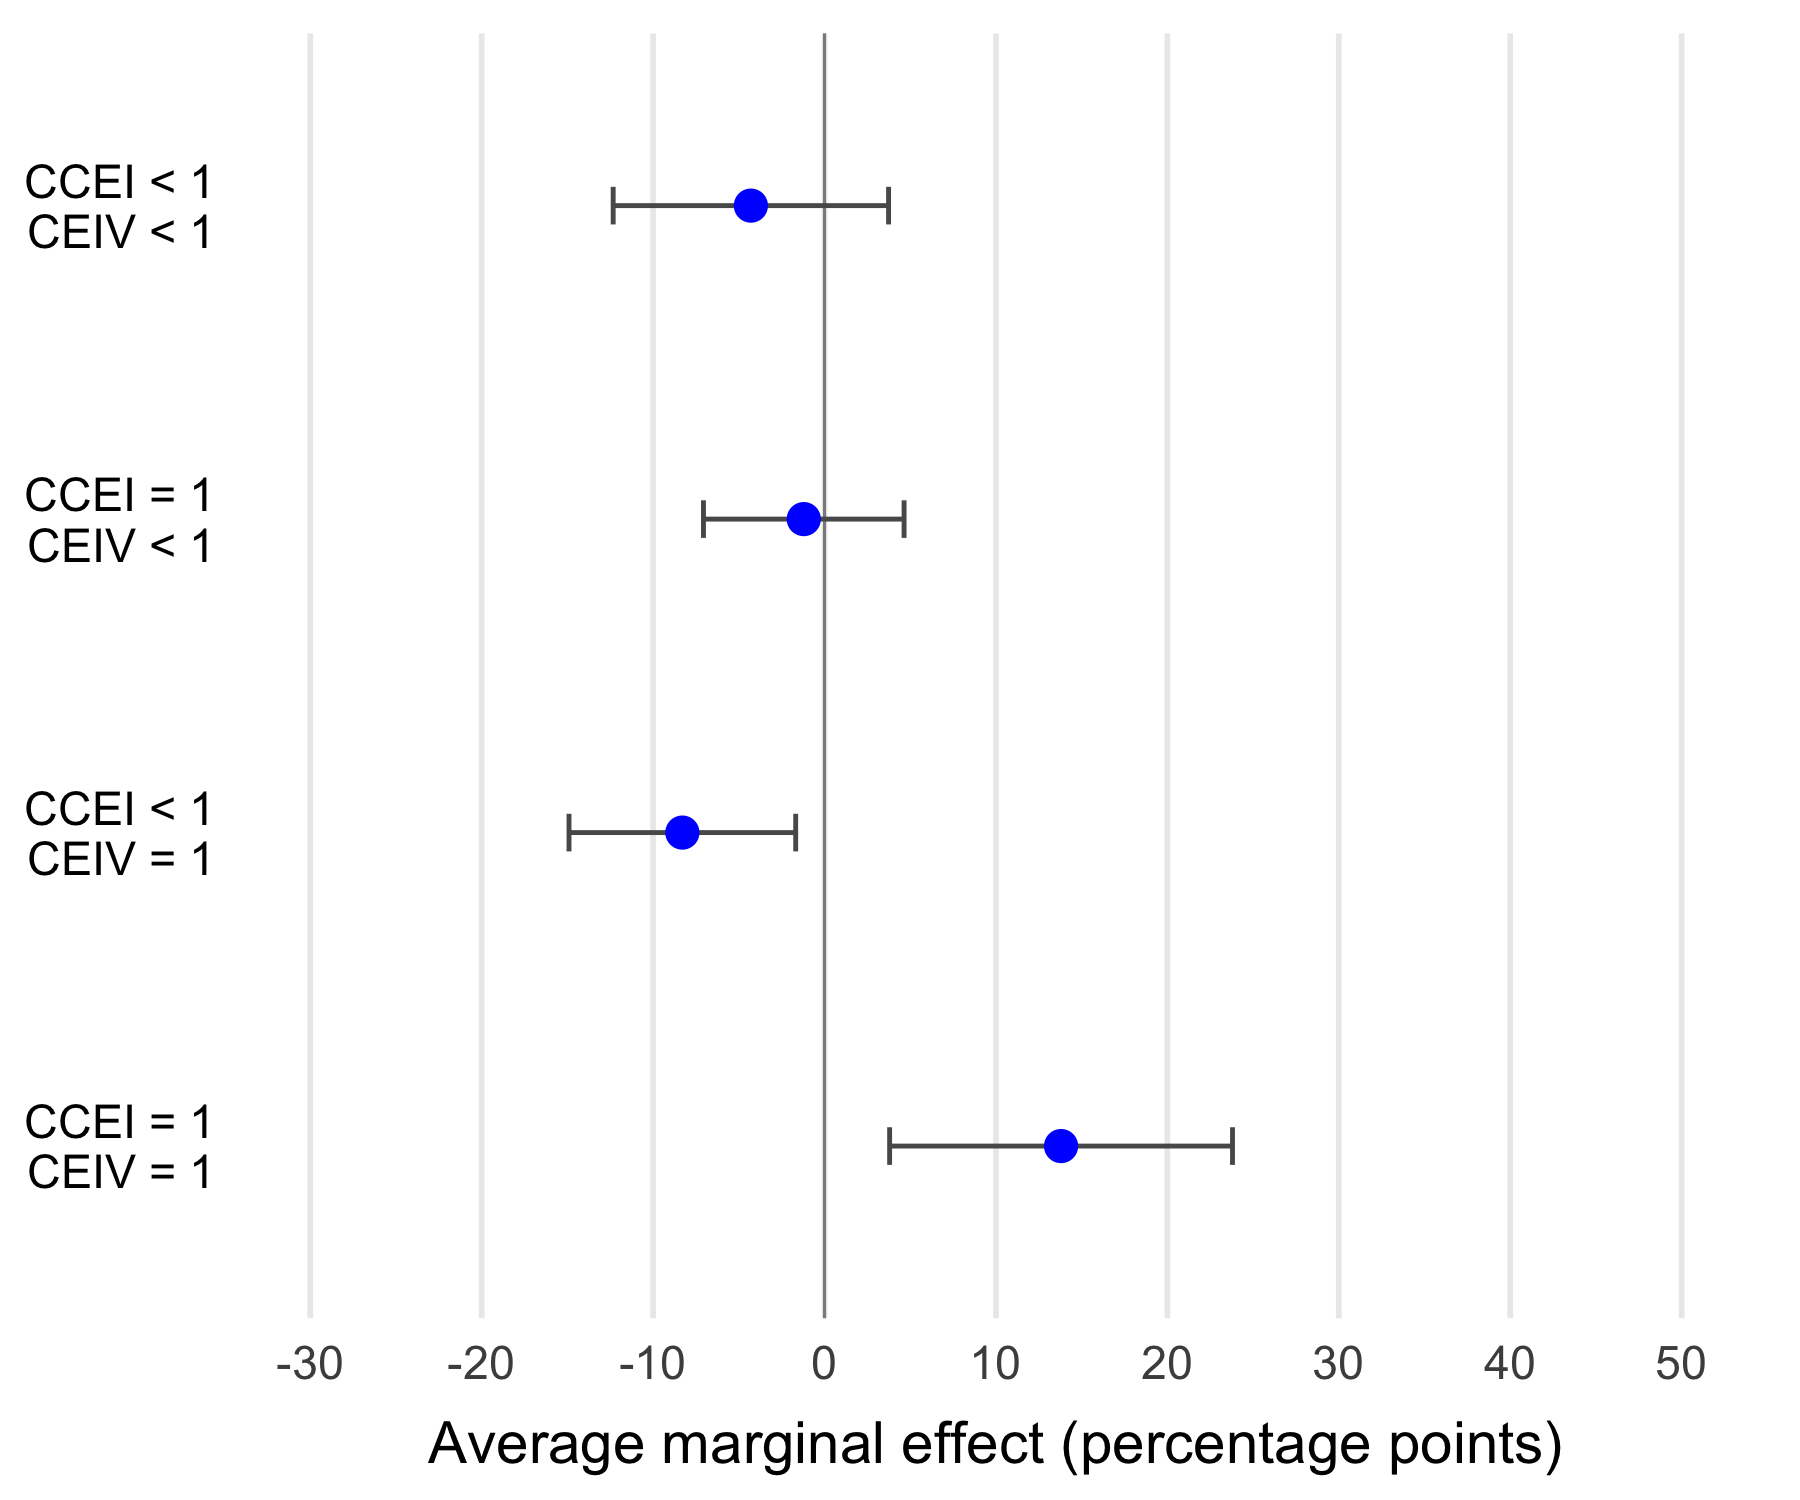
\includegraphics[width=\linewidth]{figure6_a_math_pair_0_ame_maximum.png}
\textbf{(a) More rational member: maximum CCEI}\end{minipage}\hfill\begin{minipage}{0.48\textwidth}\centering
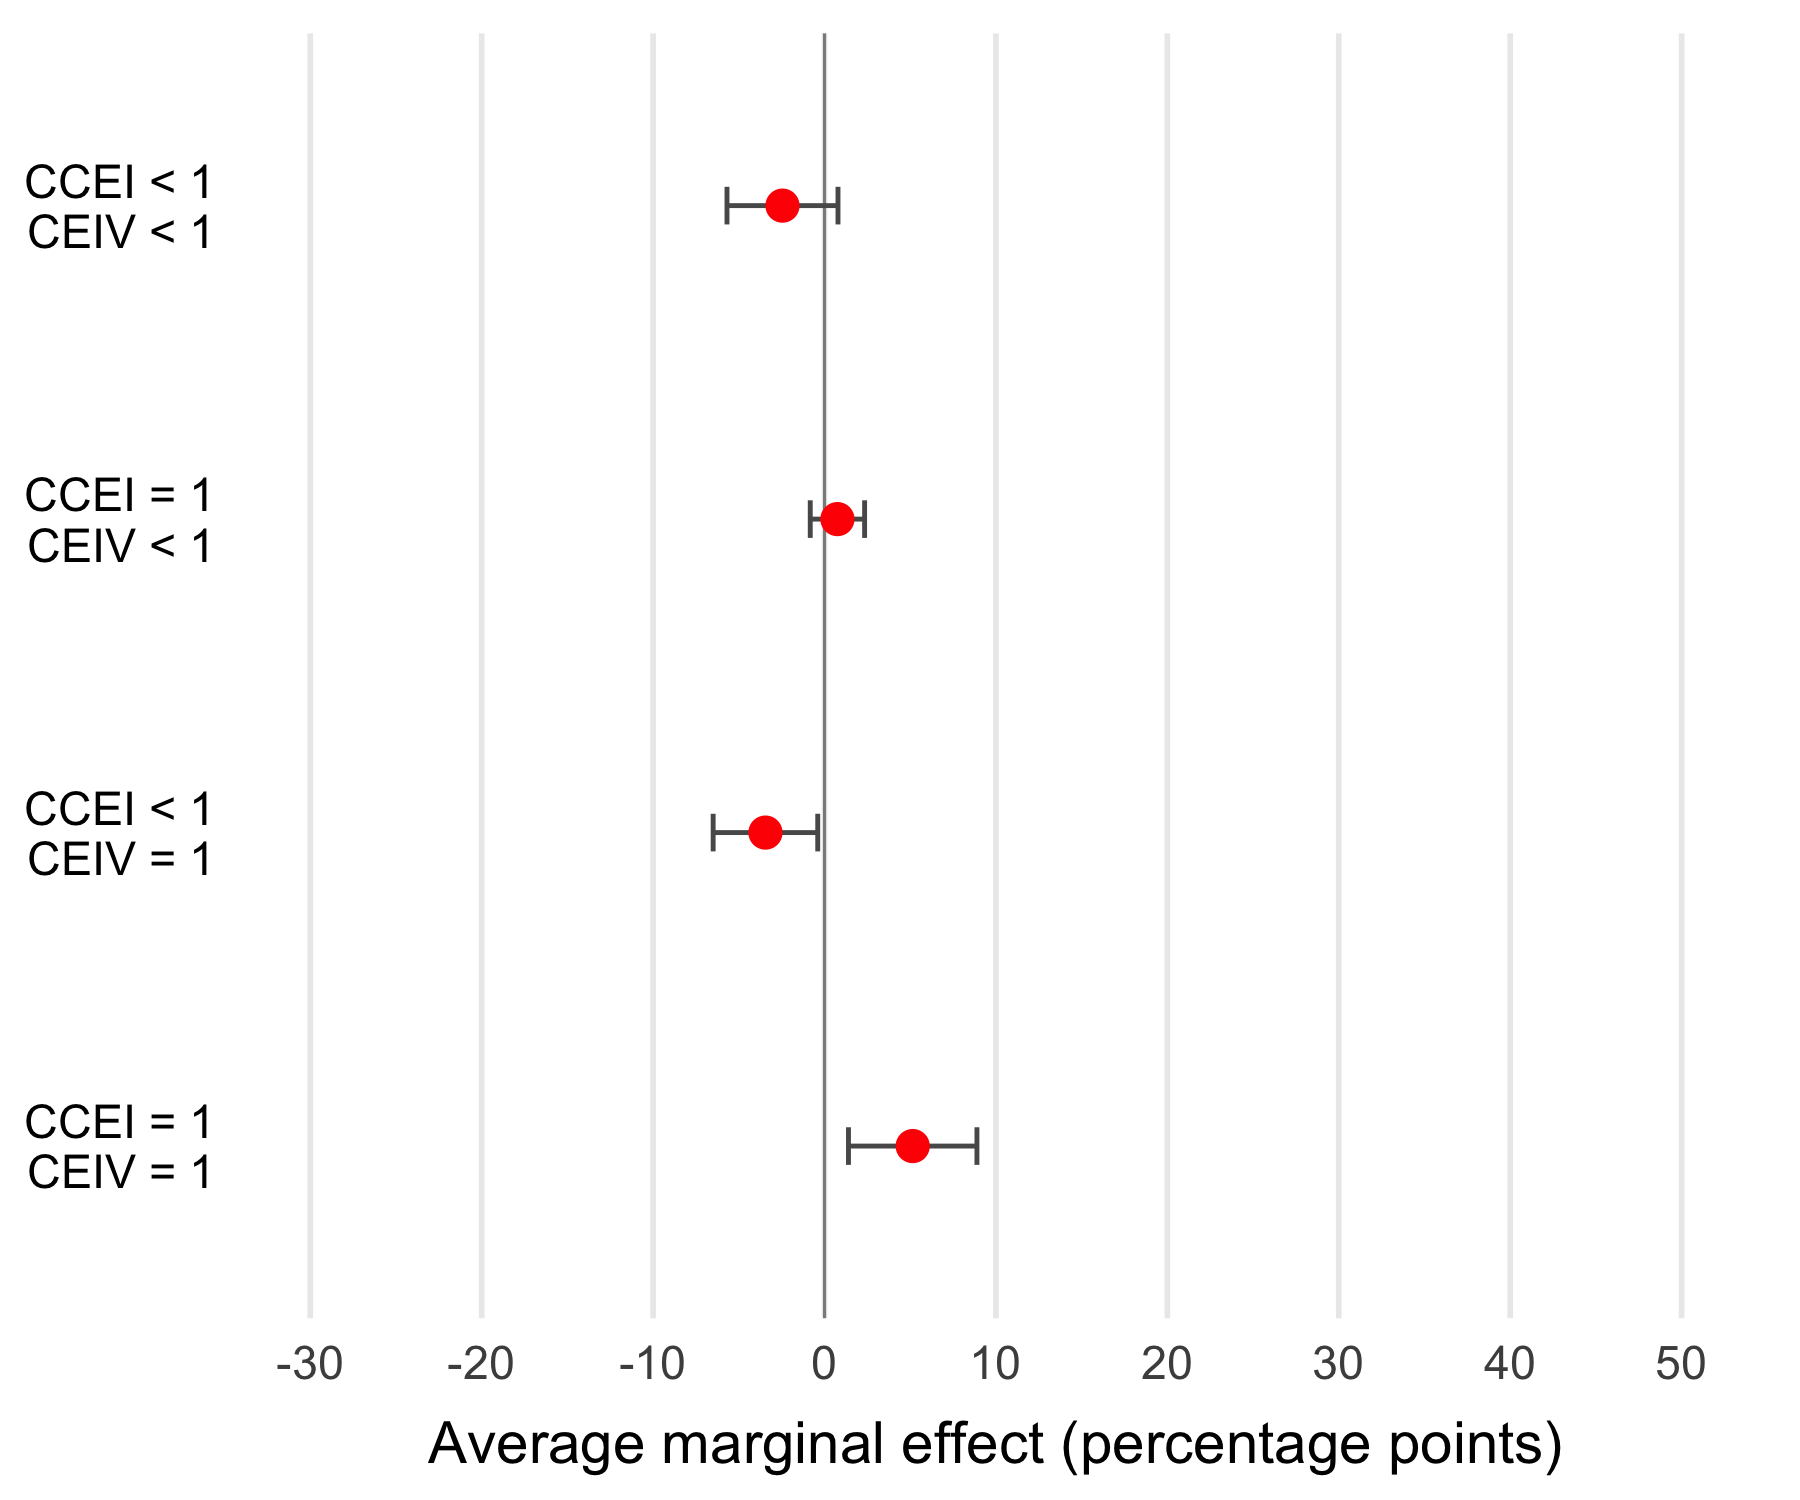
\includegraphics[width=\linewidth]{figure6_a_math_pair_0_ame_minimum.png}
\textbf{(b) Less rational member: minimum CCEI}\end{minipage}\end{center}
\begin{center}\begin{tabular}{lrrrr}\toprule
Outcome & CCEI $<1$, CEIV $<1$ & CCEI $=1$, CEIV $<1$ & CCEI $<1$, CEIV $=1$ & CCEI $=1$, CEIV $=1$\\\midrule
Observed pair-waves & 175 & 43 & 123 & 189\\
Share & 33.0\% & 8.1\% & 23.2\% & 35.7\%\\\bottomrule\end{tabular}\end{center}
\footnotesize\textit{Notes:} Effects are percentage points per 0.1 increase in individual CCEI, holding the other member's CCEI and controls fixed locally, then averaging over this subgroup. Four-category effects sum to zero for each member. Intervals use class-clustered standard errors. The class effects, coefficients, and outcome distributions can differ across separate fits; visual comparisons are descriptive.
\clearpage
\begin{center}\Large\textbf{Pair-average math: at or above wave median}\end{center}
\small Average both observed math scores (0--5); exclude 13 pair-waves with a missing score. Wave medians are 2.5 at baseline and 3 at endline. Median ties enter the higher bin; eligible low/high counts are 530/761.
Separate-subgroup fit: 761 pair-waves, 487 distinct pairs, 64 class clusters.
\begin{center}\begin{minipage}{0.48\textwidth}\centering
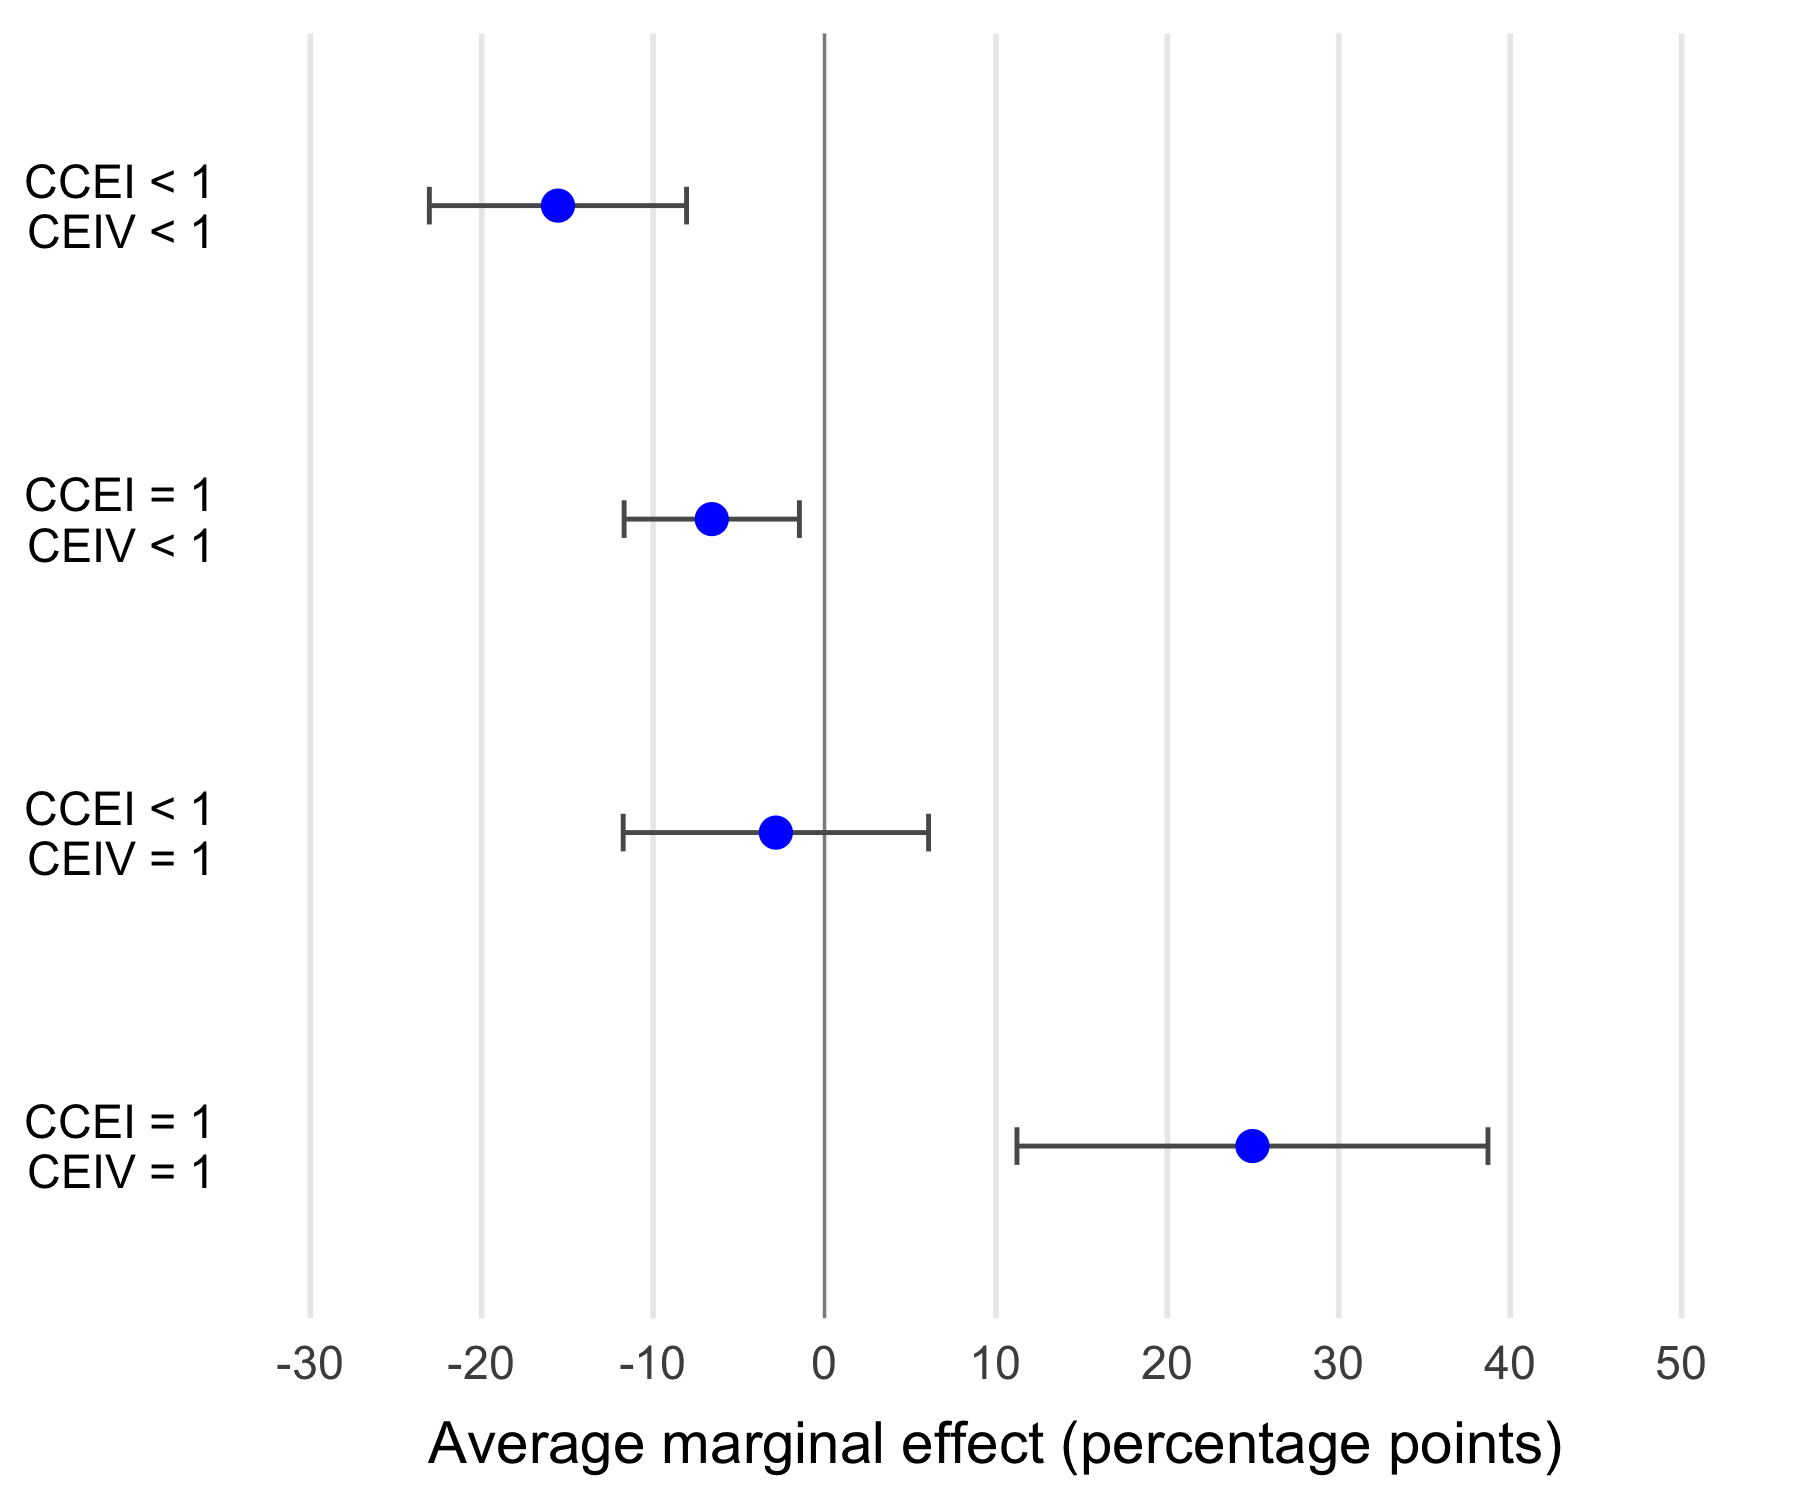
\includegraphics[width=\linewidth]{figure6_a_math_pair_1_ame_maximum.png}
\textbf{(a) More rational member: maximum CCEI}\end{minipage}\hfill\begin{minipage}{0.48\textwidth}\centering
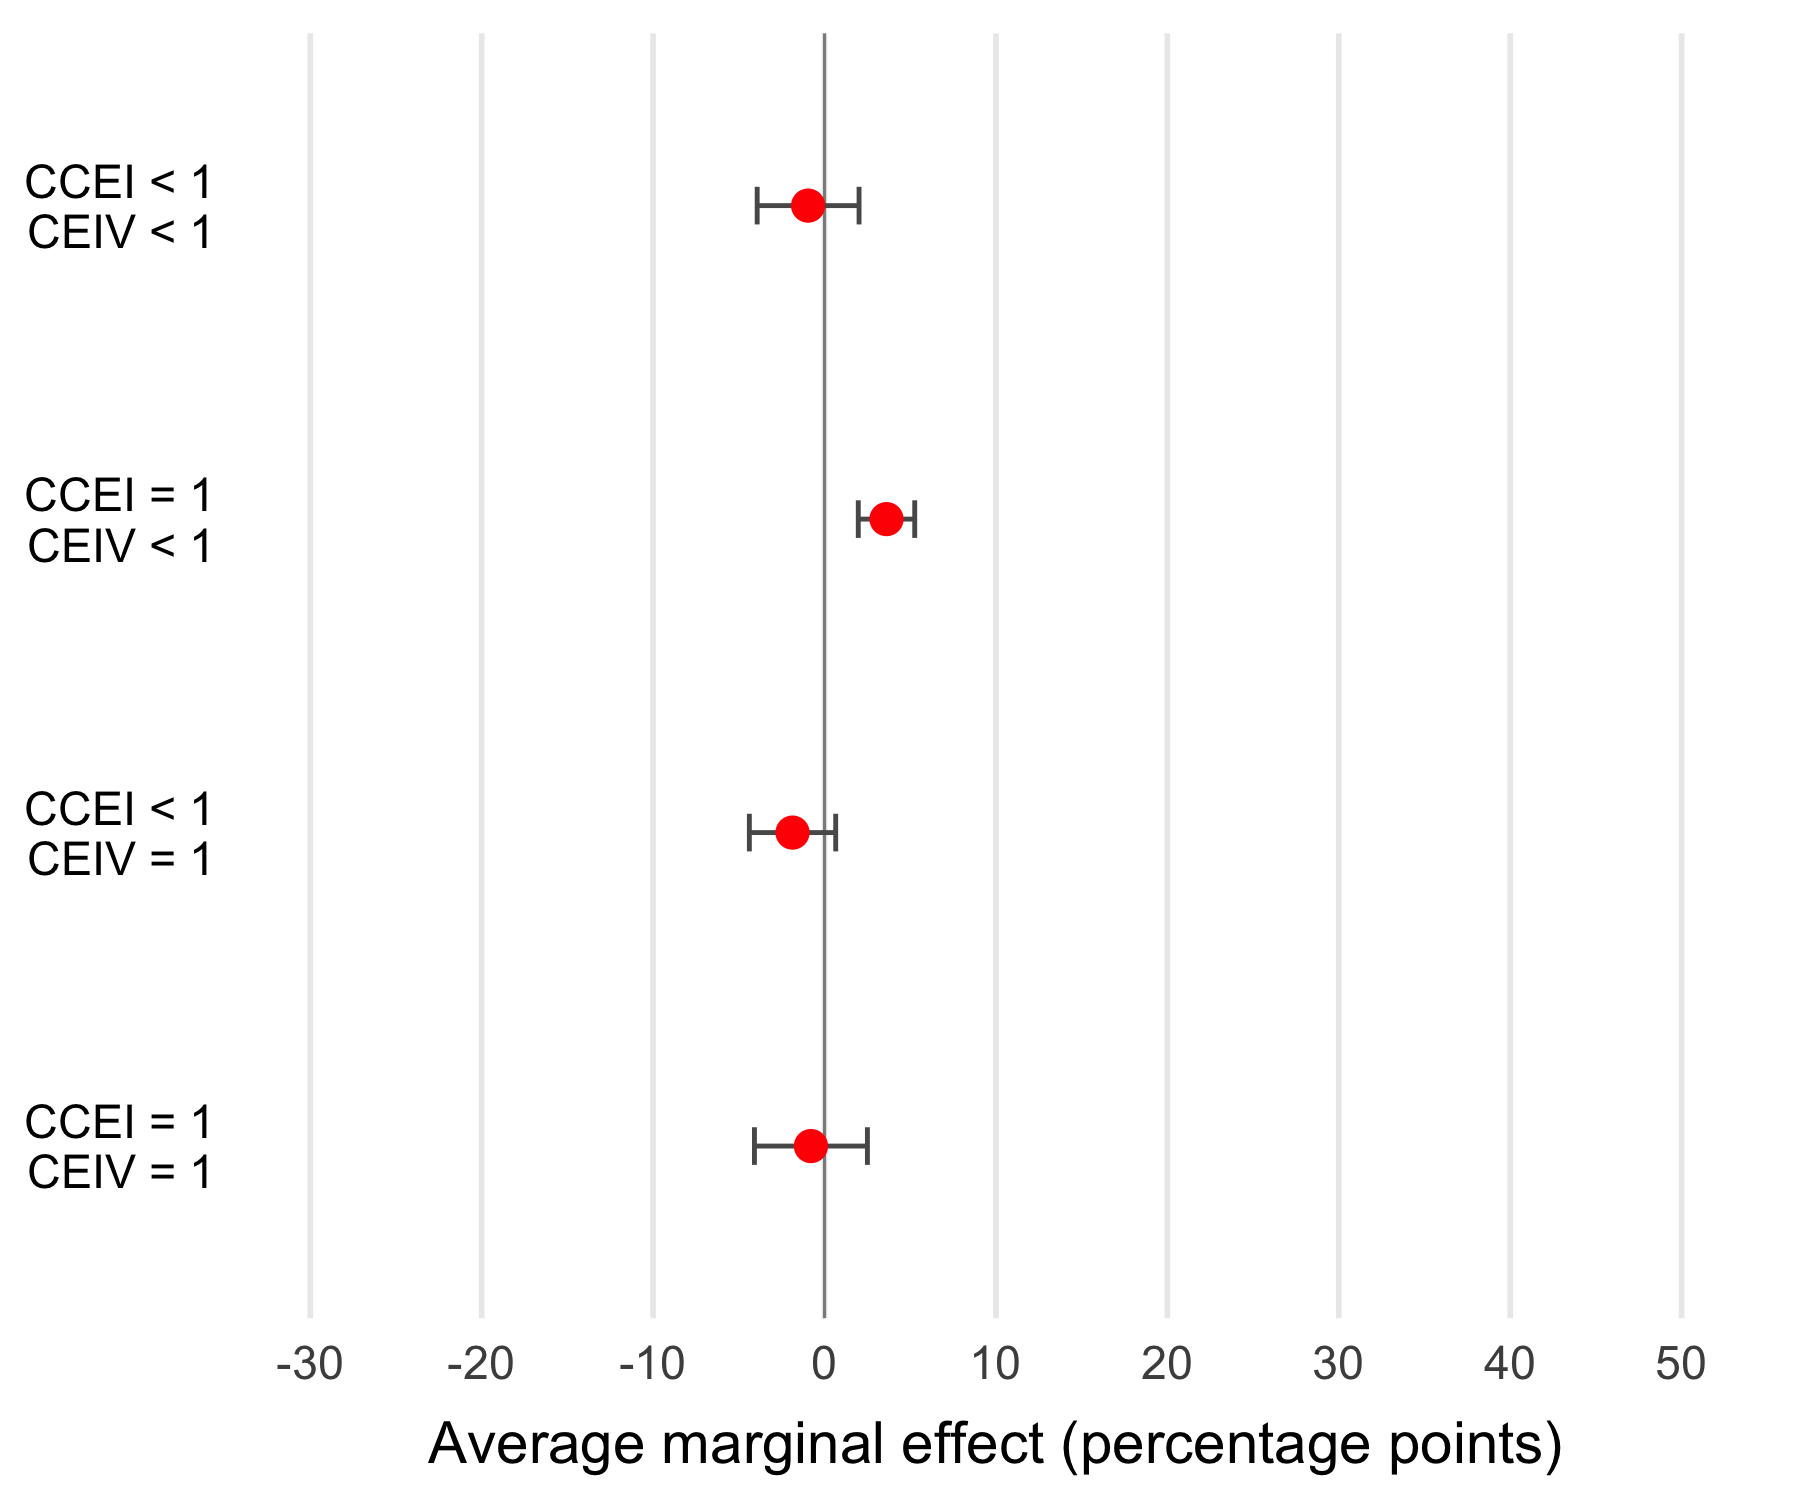
\includegraphics[width=\linewidth]{figure6_a_math_pair_1_ame_minimum.png}
\textbf{(b) Less rational member: minimum CCEI}\end{minipage}\end{center}
\begin{center}\begin{tabular}{lrrrr}\toprule
Outcome & CCEI $<1$, CEIV $<1$ & CCEI $=1$, CEIV $<1$ & CCEI $<1$, CEIV $=1$ & CCEI $=1$, CEIV $=1$\\\midrule
Observed pair-waves & 237 & 71 & 172 & 281\\
Share & 31.1\% & 9.3\% & 22.6\% & 36.9\%\\\bottomrule\end{tabular}\end{center}
\footnotesize\textit{Notes:} Effects are percentage points per 0.1 increase in individual CCEI, holding the other member's CCEI and controls fixed locally, then averaging over this subgroup. Four-category effects sum to zero for each member. Intervals use class-clustered standard errors. The class effects, coefficients, and outcome distributions can differ across separate fits; visual comparisons are descriptive.
\clearpage
\begin{center}\Large\textbf{Less rational member's math: below wave median}\end{center}
\small Select the member with strictly lower individual CCEI in each wave. Exclude 199 CCEI-tied pair-waves and 11 additional pair-waves with missing selected-member math. The median is 3 in both waves; ties enter the higher bin. Eligible low/high counts are 522/572. The selected member can change across waves.
Separate-subgroup fit: 522 pair-waves, 385 distinct pairs, 63 class clusters.
\begin{center}\begin{minipage}{0.48\textwidth}\centering
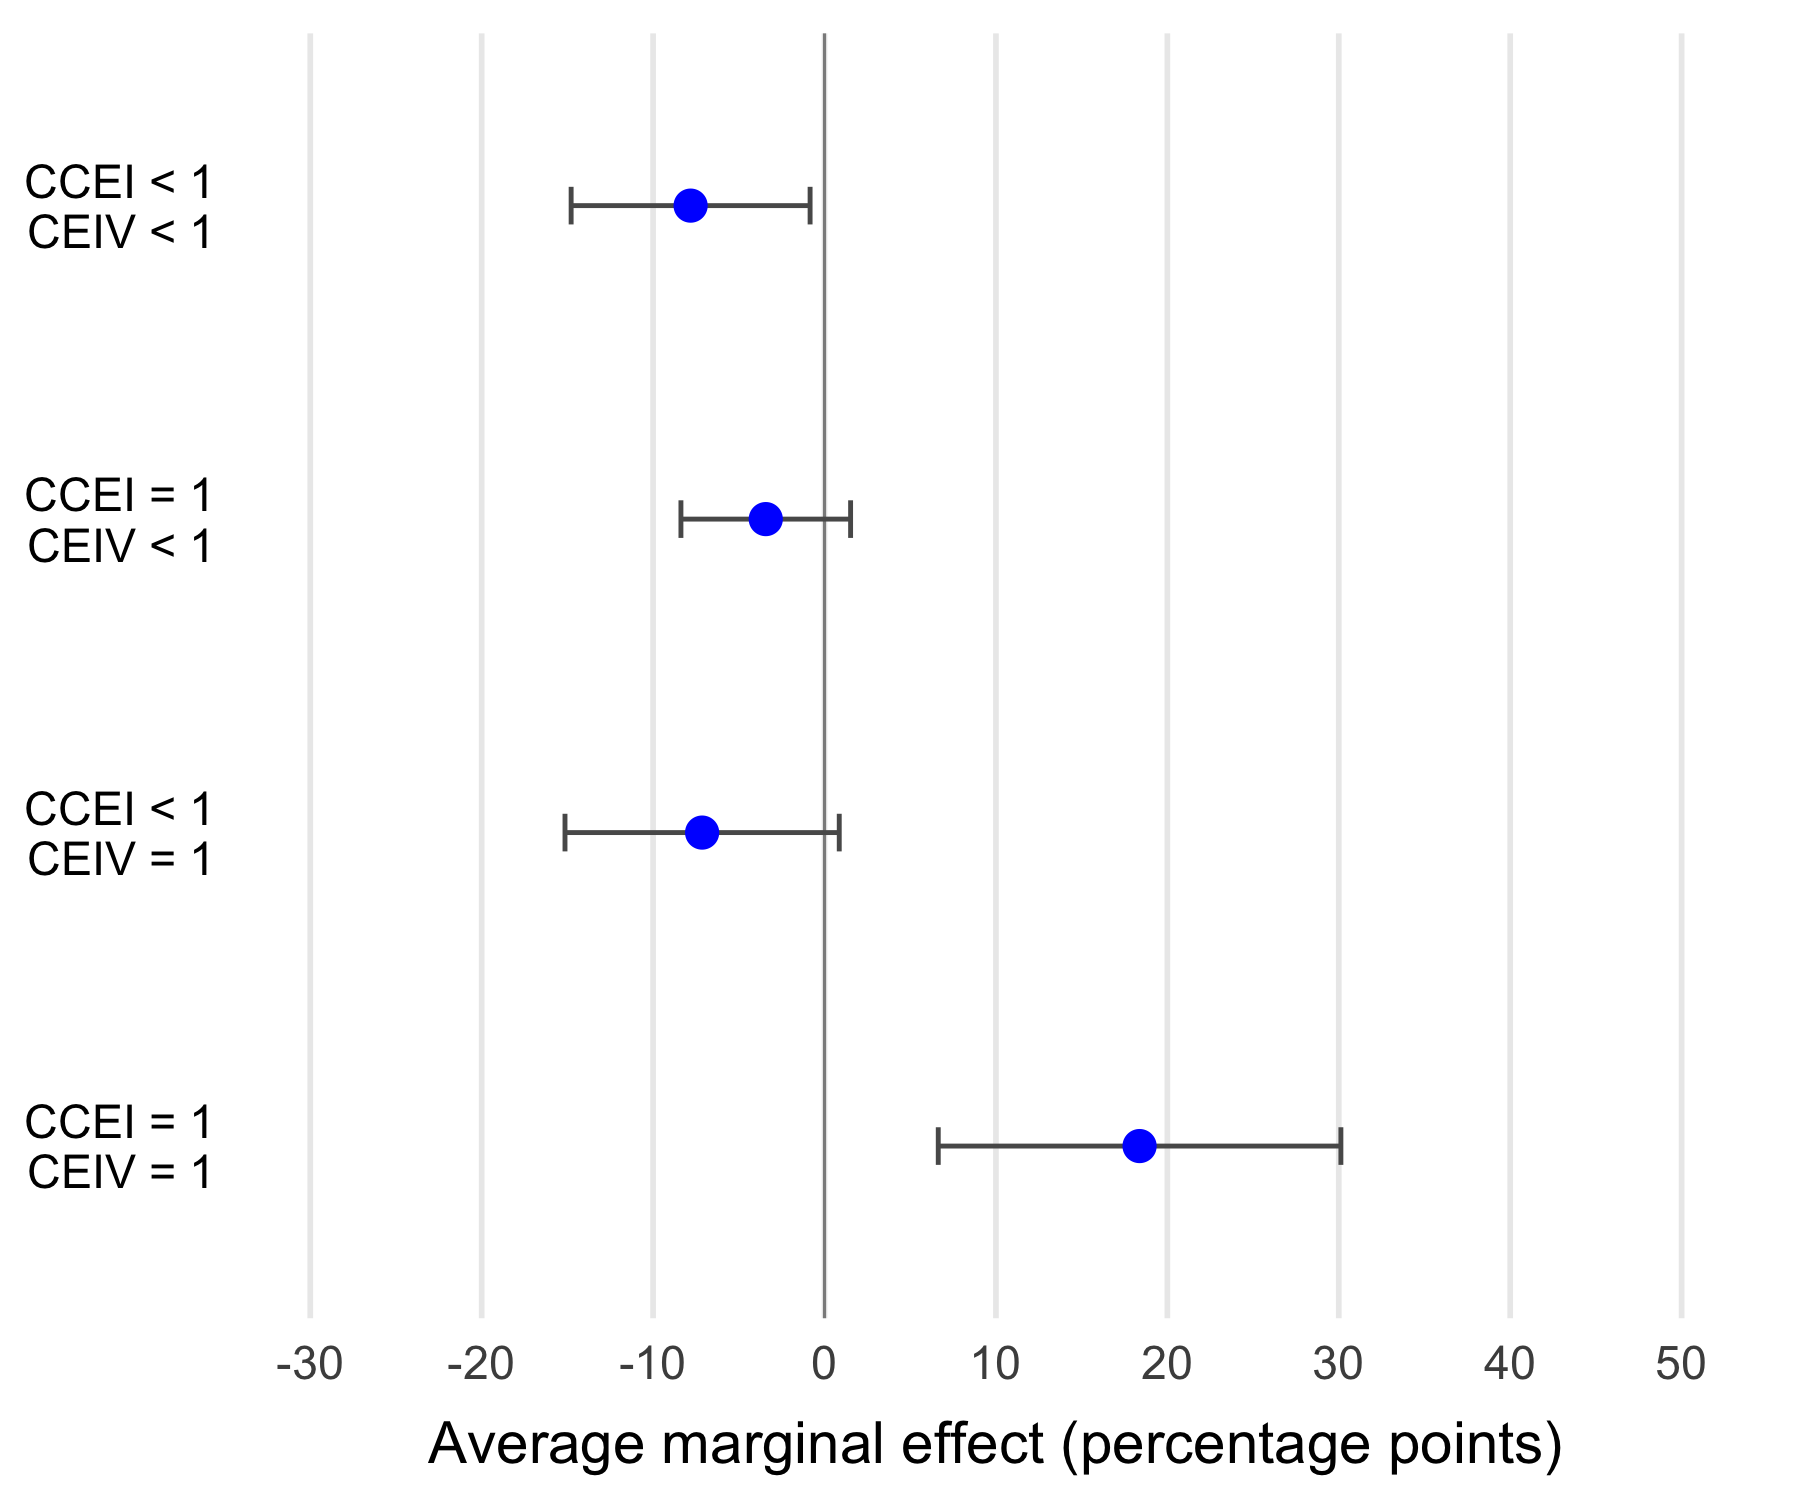
\includegraphics[width=\linewidth]{figure6_a_math_less_0_ame_maximum.png}
\textbf{(a) More rational member: maximum CCEI}\end{minipage}\hfill\begin{minipage}{0.48\textwidth}\centering
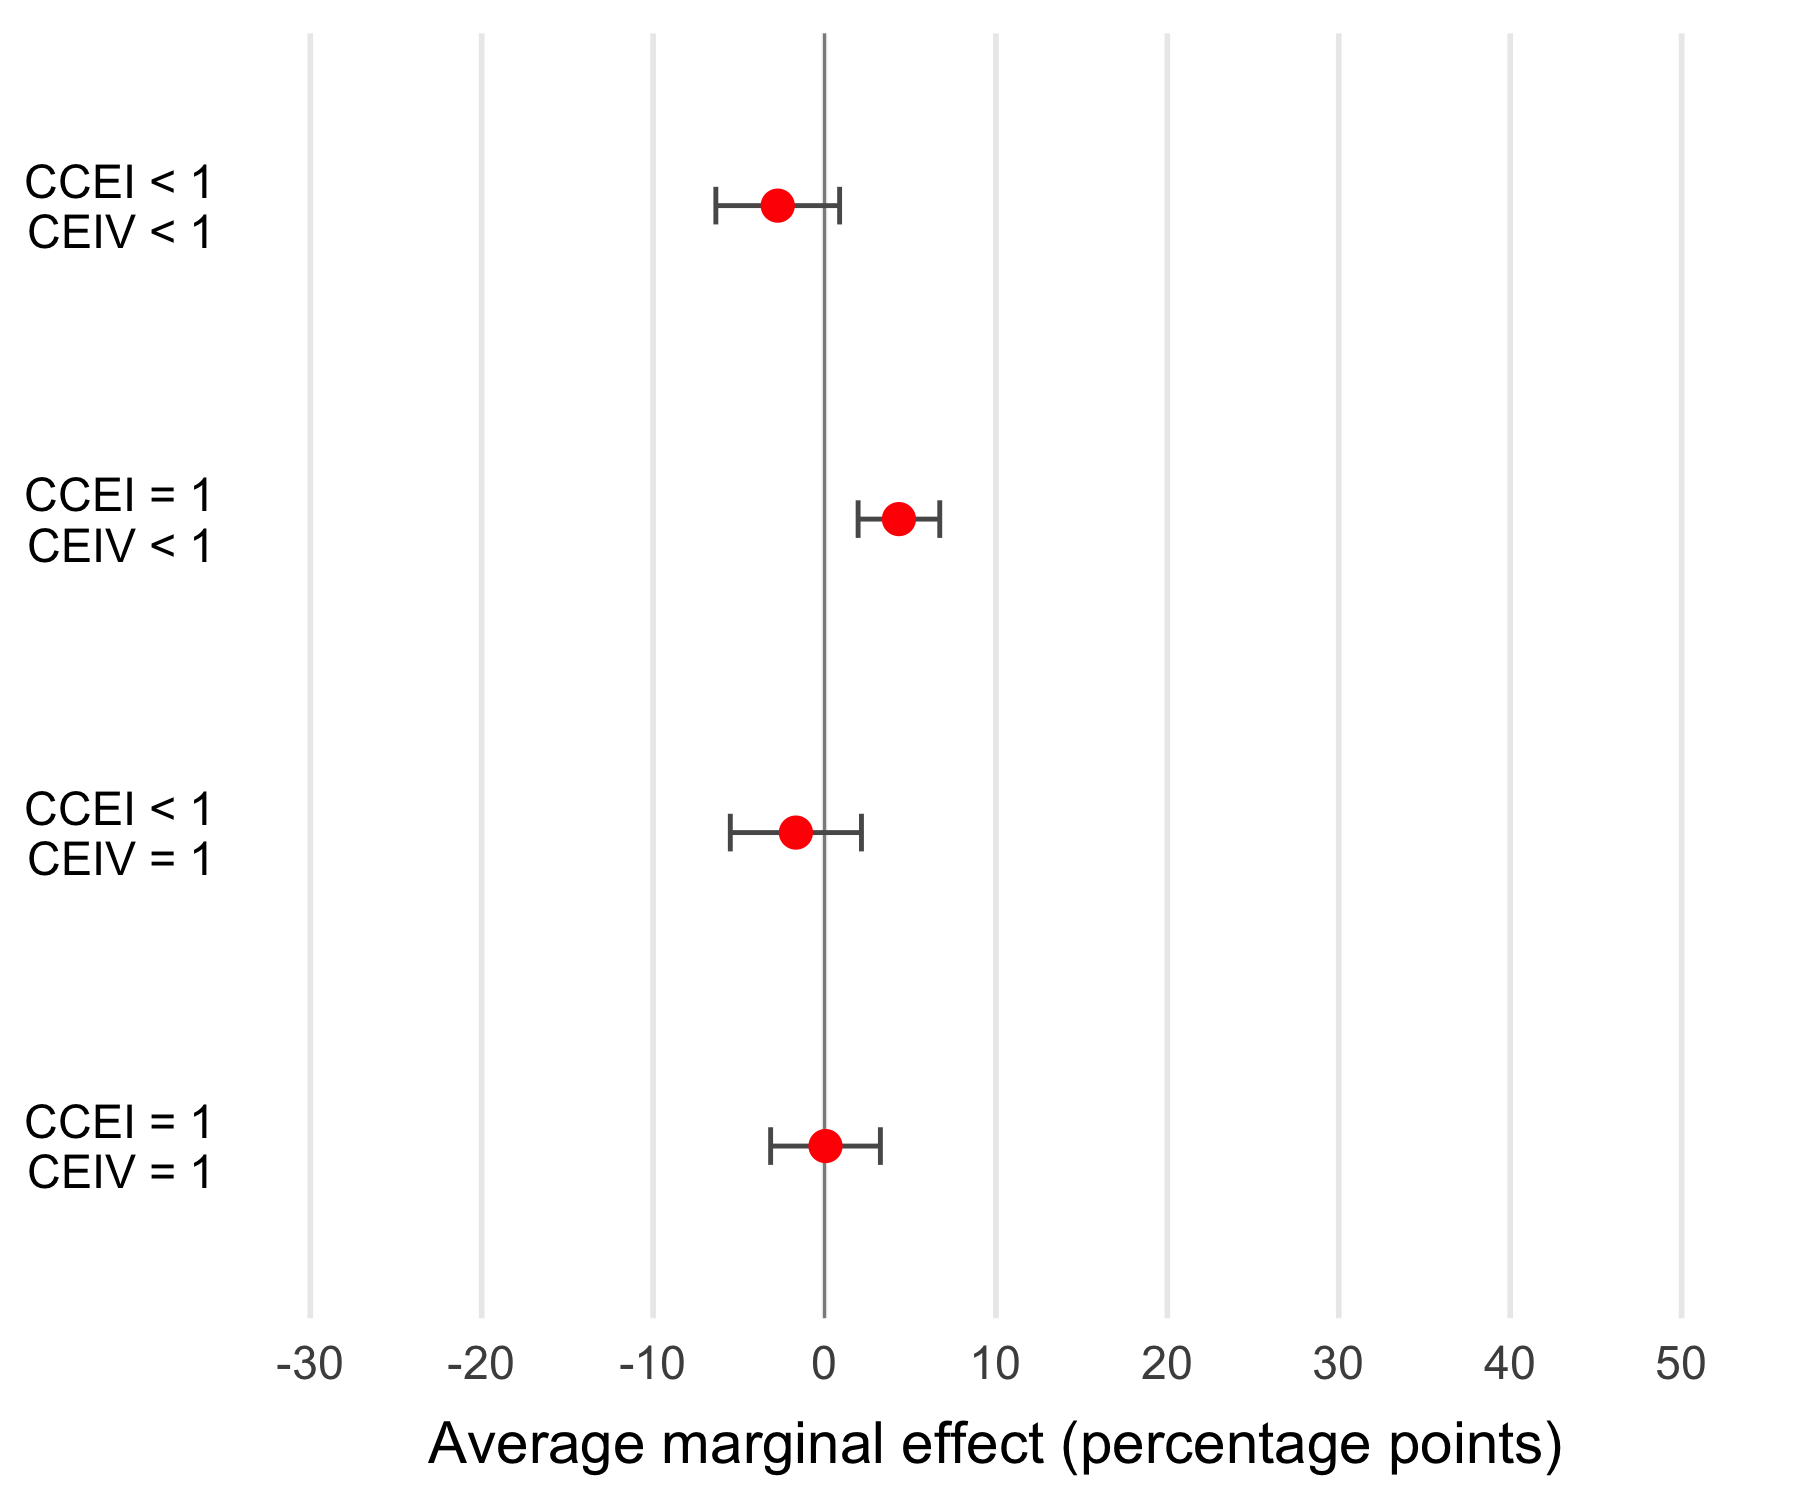
\includegraphics[width=\linewidth]{figure6_a_math_less_0_ame_minimum.png}
\textbf{(b) Less rational member: minimum CCEI}\end{minipage}\end{center}
\begin{center}\begin{tabular}{lrrrr}\toprule
Outcome & CCEI $<1$, CEIV $<1$ & CCEI $=1$, CEIV $<1$ & CCEI $<1$, CEIV $=1$ & CCEI $=1$, CEIV $=1$\\\midrule
Observed pair-waves & 187 & 47 & 128 & 160\\
Share & 35.8\% & 9.0\% & 24.5\% & 30.7\%\\\bottomrule\end{tabular}\end{center}
\footnotesize\textit{Notes:} Effects are percentage points per 0.1 increase in individual CCEI, holding the other member's CCEI and controls fixed locally, then averaging over this subgroup. Four-category effects sum to zero for each member. Intervals use class-clustered standard errors. The class effects, coefficients, and outcome distributions can differ across separate fits; visual comparisons are descriptive.
\clearpage
\begin{center}\Large\textbf{Less rational member's math: at or above wave median}\end{center}
\small Select the member with strictly lower individual CCEI in each wave. Exclude 199 CCEI-tied pair-waves and 11 additional pair-waves with missing selected-member math. The median is 3 in both waves; ties enter the higher bin. Eligible low/high counts are 522/572. The selected member can change across waves.
Separate-subgroup fit: 572 pair-waves, 417 distinct pairs, 64 class clusters.
\begin{center}\begin{minipage}{0.48\textwidth}\centering
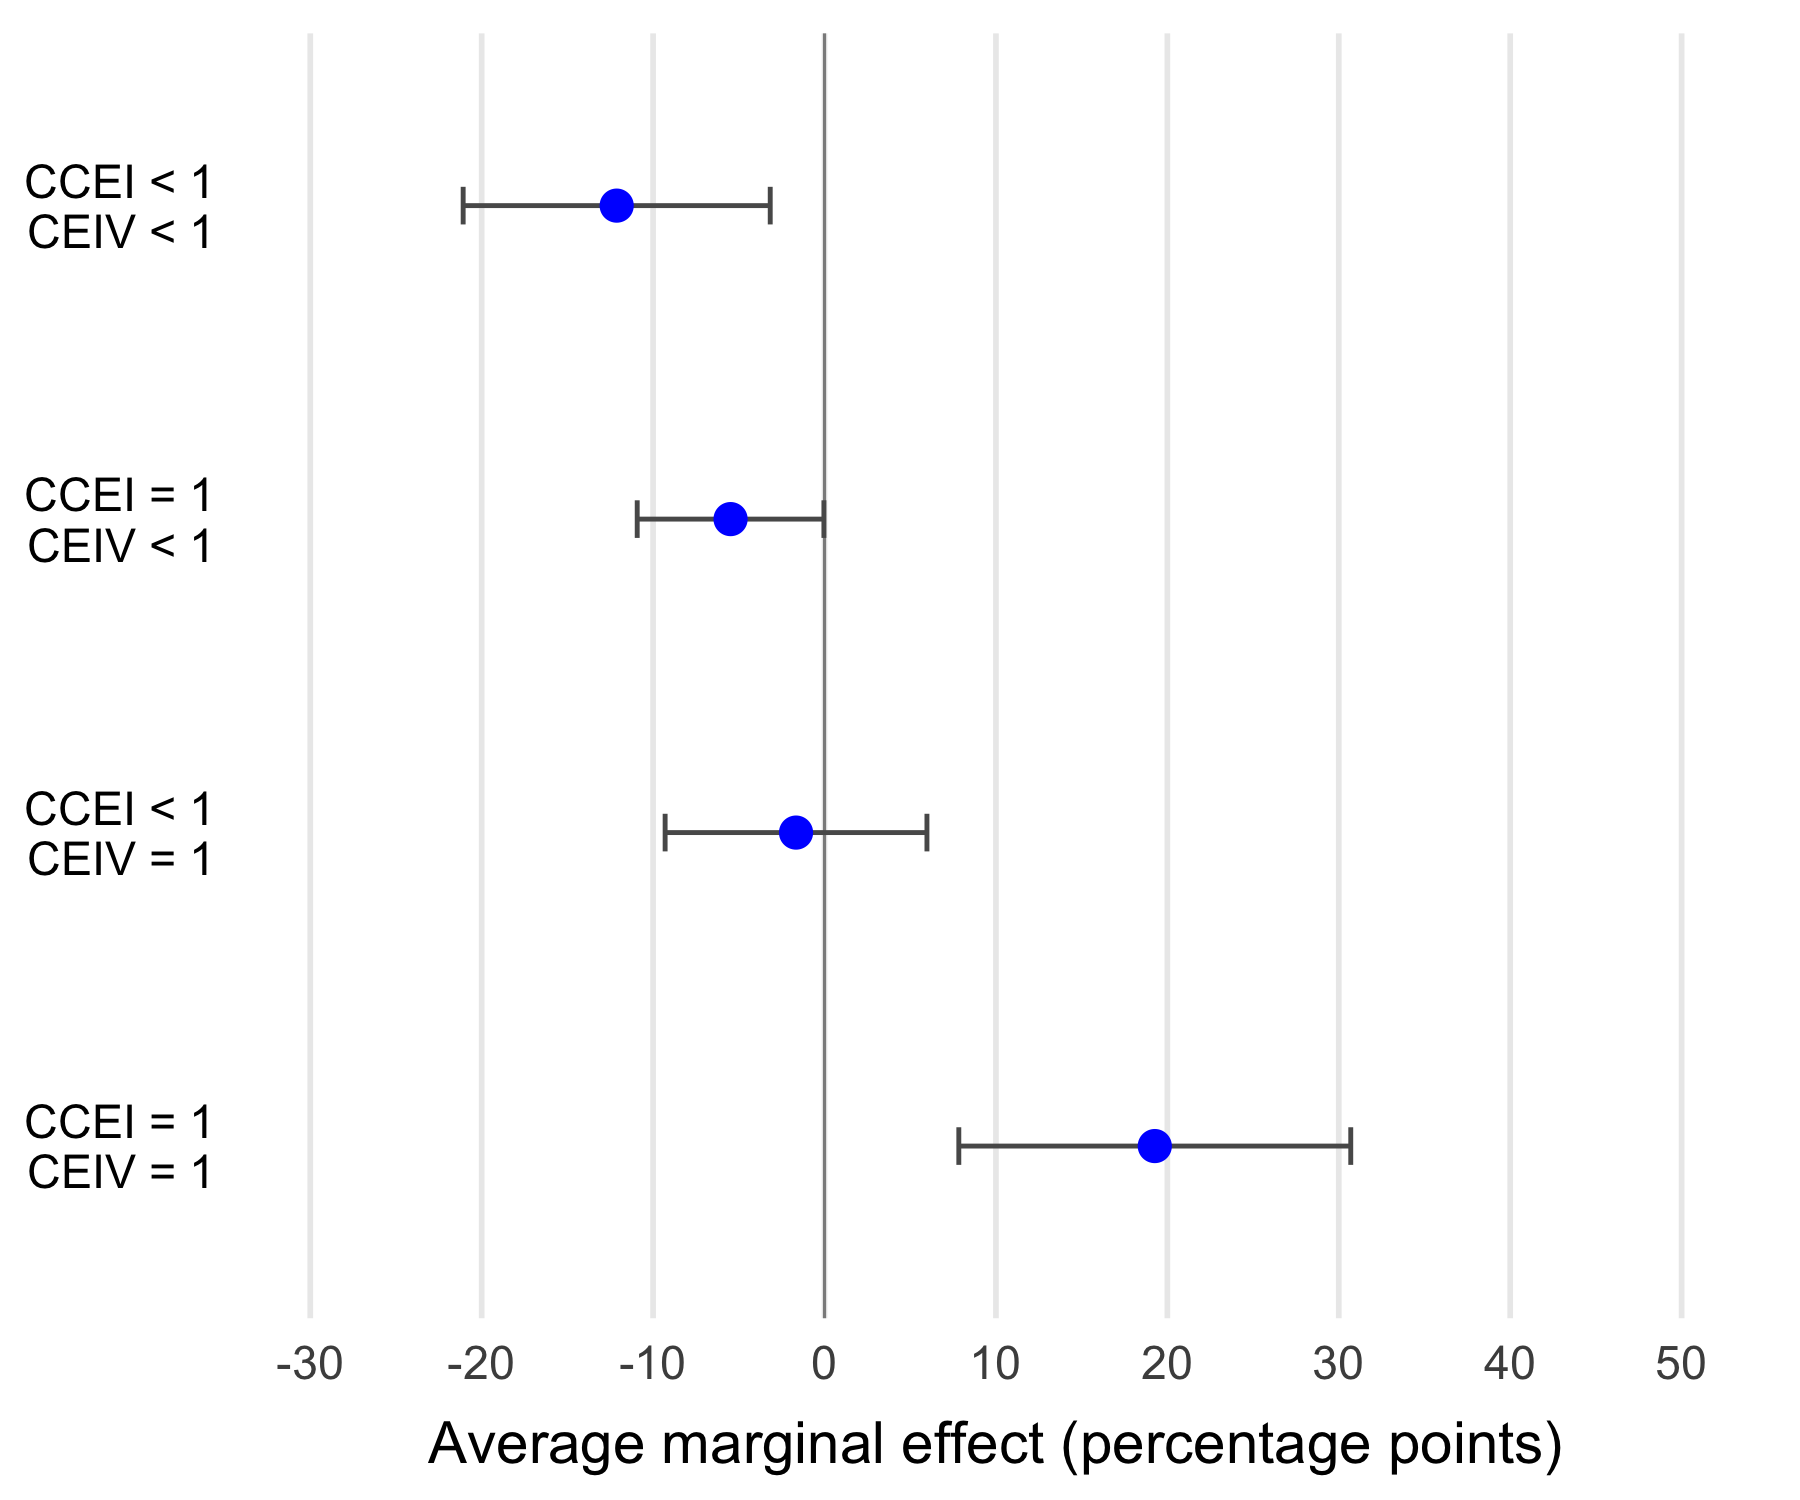
\includegraphics[width=\linewidth]{figure6_a_math_less_1_ame_maximum.png}
\textbf{(a) More rational member: maximum CCEI}\end{minipage}\hfill\begin{minipage}{0.48\textwidth}\centering
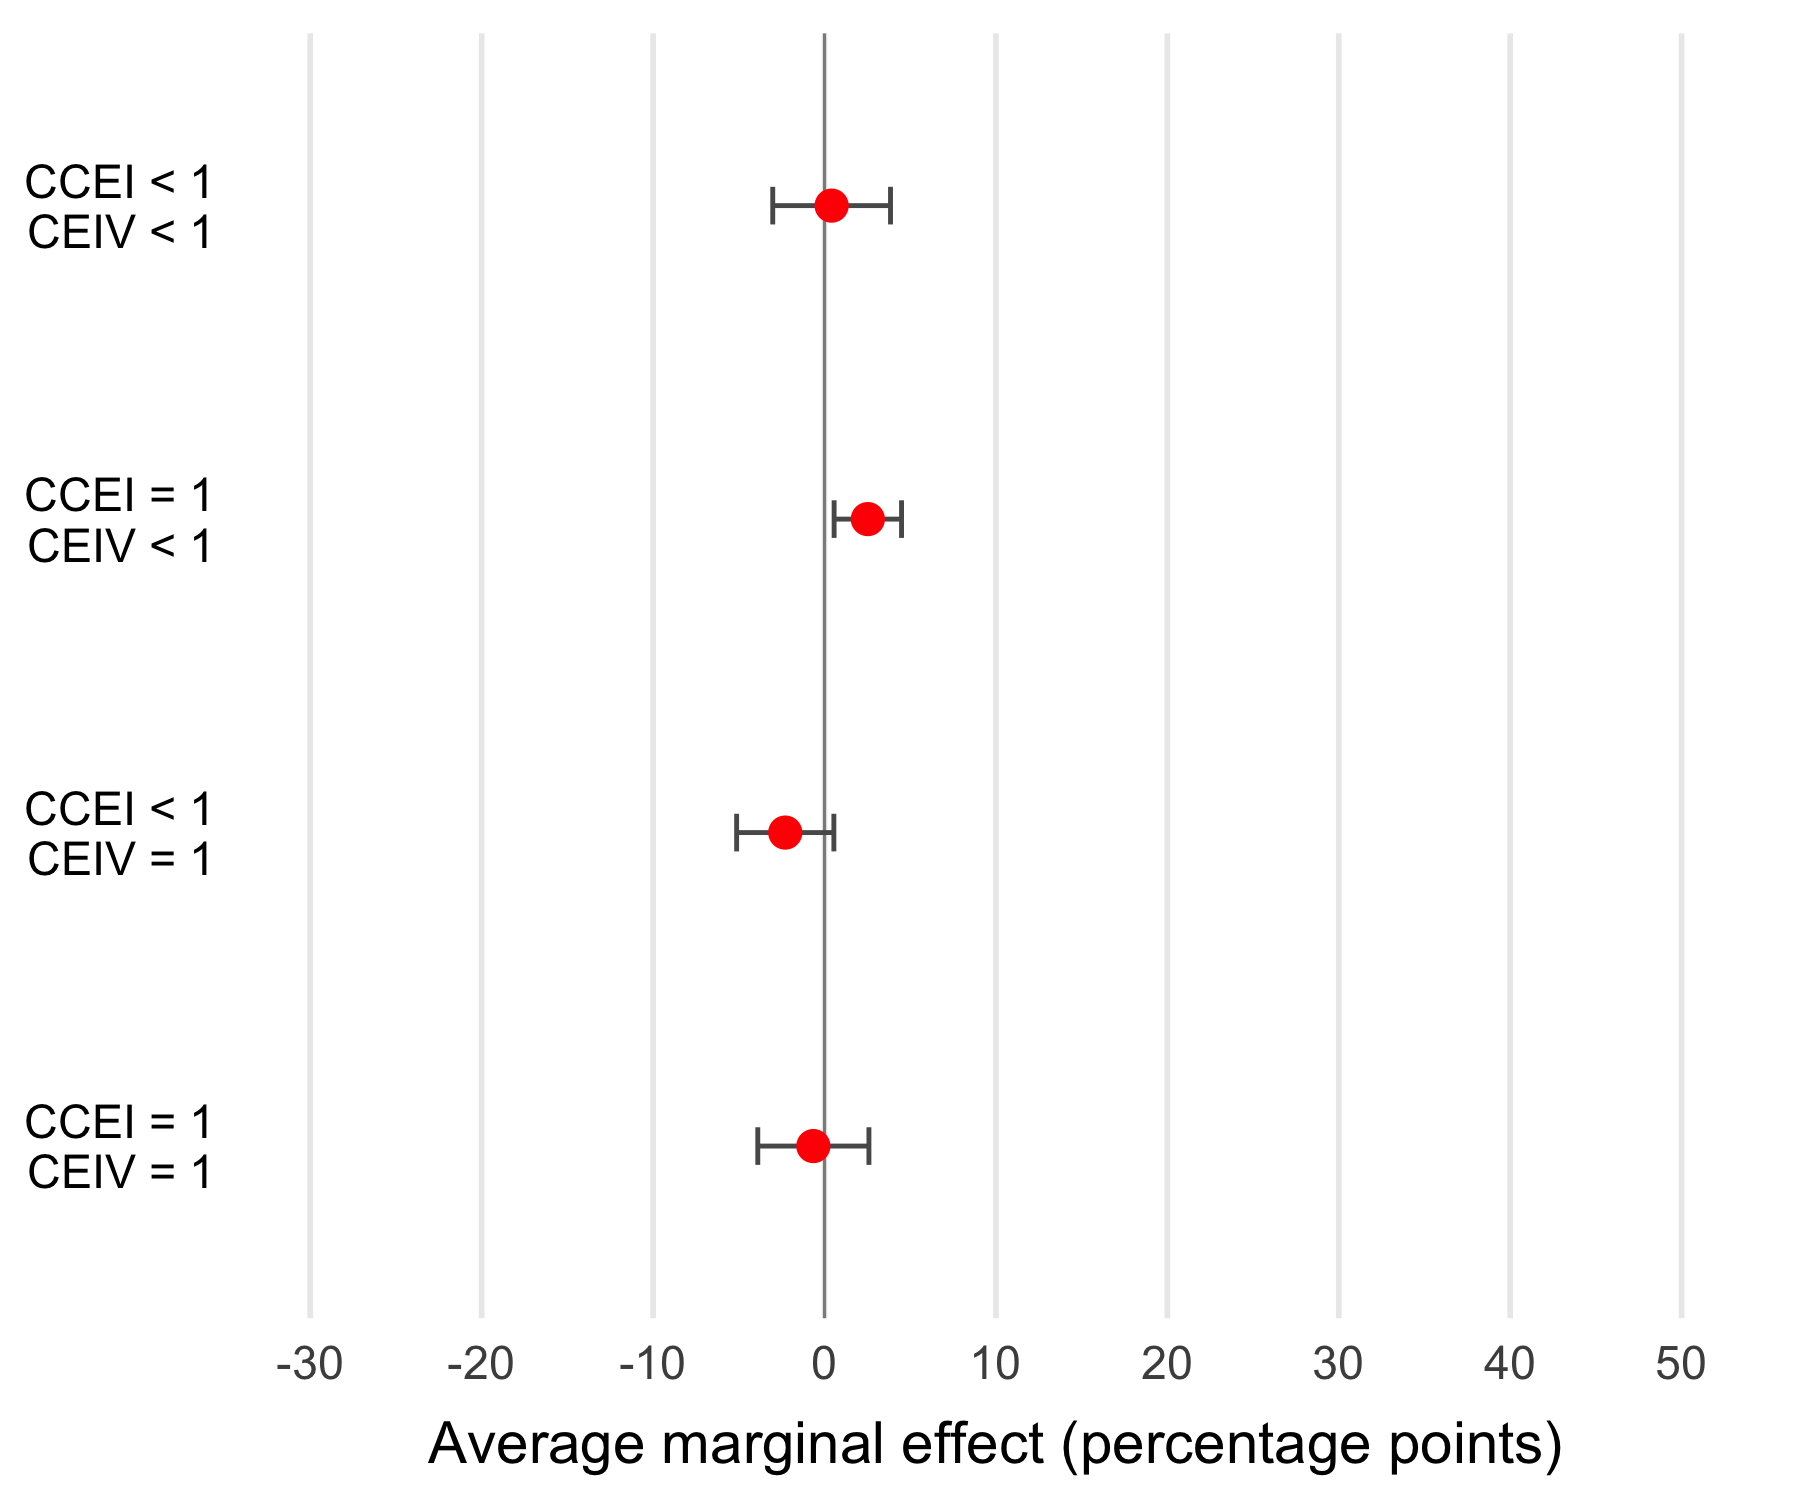
\includegraphics[width=\linewidth]{figure6_a_math_less_1_ame_minimum.png}
\textbf{(b) Less rational member: minimum CCEI}\end{minipage}\end{center}
\begin{center}\begin{tabular}{lrrrr}\toprule
Outcome & CCEI $<1$, CEIV $<1$ & CCEI $=1$, CEIV $<1$ & CCEI $<1$, CEIV $=1$ & CCEI $=1$, CEIV $=1$\\\midrule
Observed pair-waves & 189 & 51 & 136 & 196\\
Share & 33.0\% & 8.9\% & 23.8\% & 34.3\%\\\bottomrule\end{tabular}\end{center}
\footnotesize\textit{Notes:} Effects are percentage points per 0.1 increase in individual CCEI, holding the other member's CCEI and controls fixed locally, then averaging over this subgroup. Four-category effects sum to zero for each member. Intervals use class-clustered standard errors. The class effects, coefficients, and outcome distributions can differ across separate fits; visual comparisons are descriptive.
\clearpage
\begin{center}\Large\textbf{No friendship nomination: three-category reference}\end{center}
\small Directed friendship nominations distinguish none, one-sided, and mutual. Eligible counts are 912/225/167 pair-waves. The no-nomination figure duplicates the corresponding binary-friendship reference.
Separate-subgroup fit: 912 pair-waves, 518 distinct pairs, 64 class clusters.
\begin{center}\begin{minipage}{0.48\textwidth}\centering
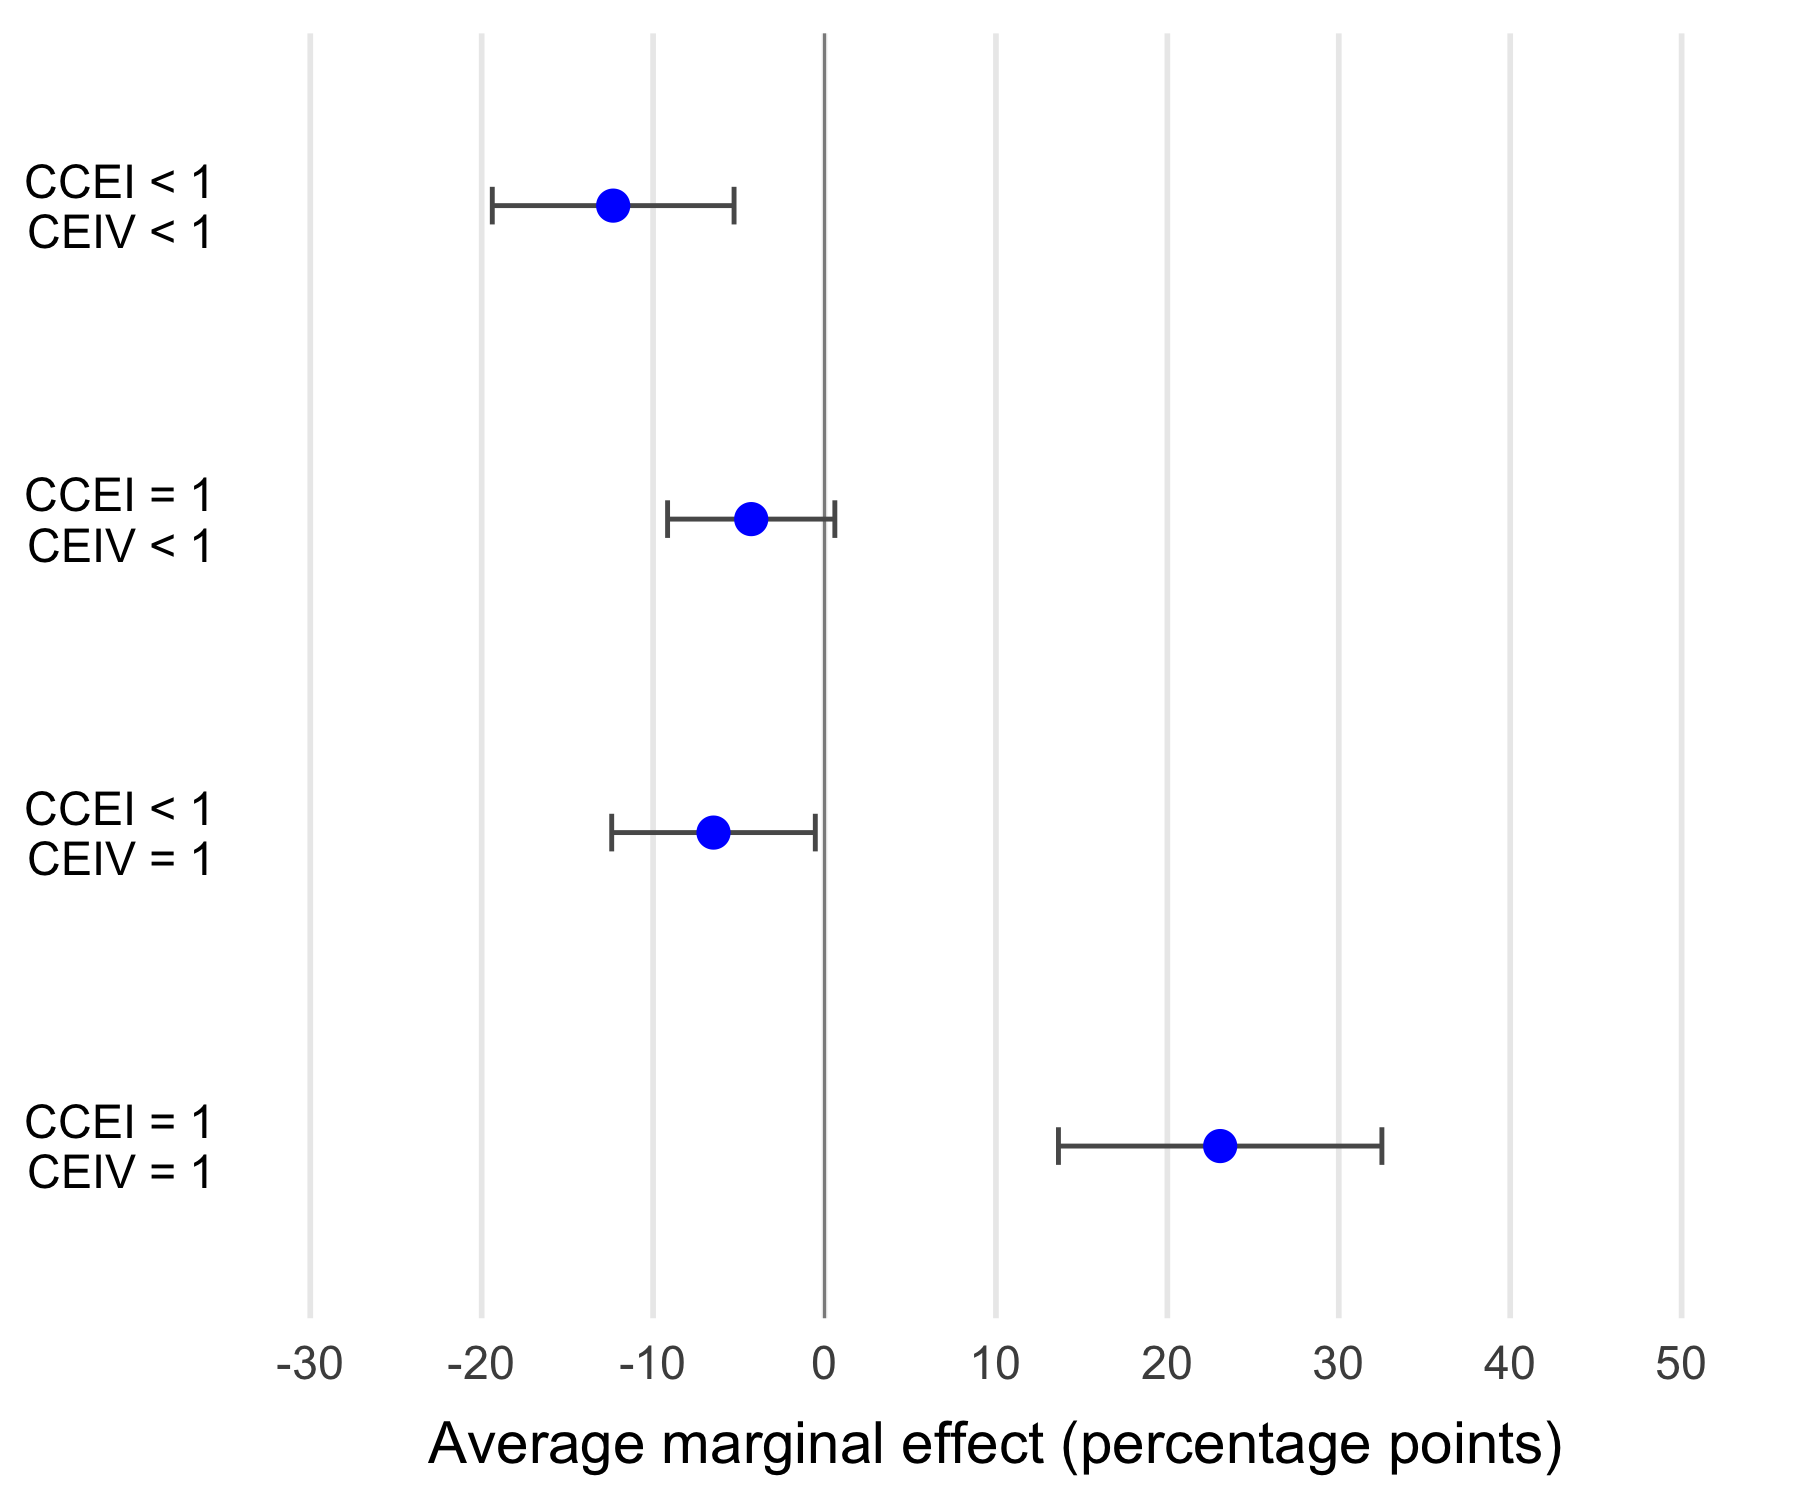
\includegraphics[width=\linewidth]{figure6_a_friend_0_ame_maximum.png}
\textbf{(a) More rational member: maximum CCEI}\end{minipage}\hfill\begin{minipage}{0.48\textwidth}\centering
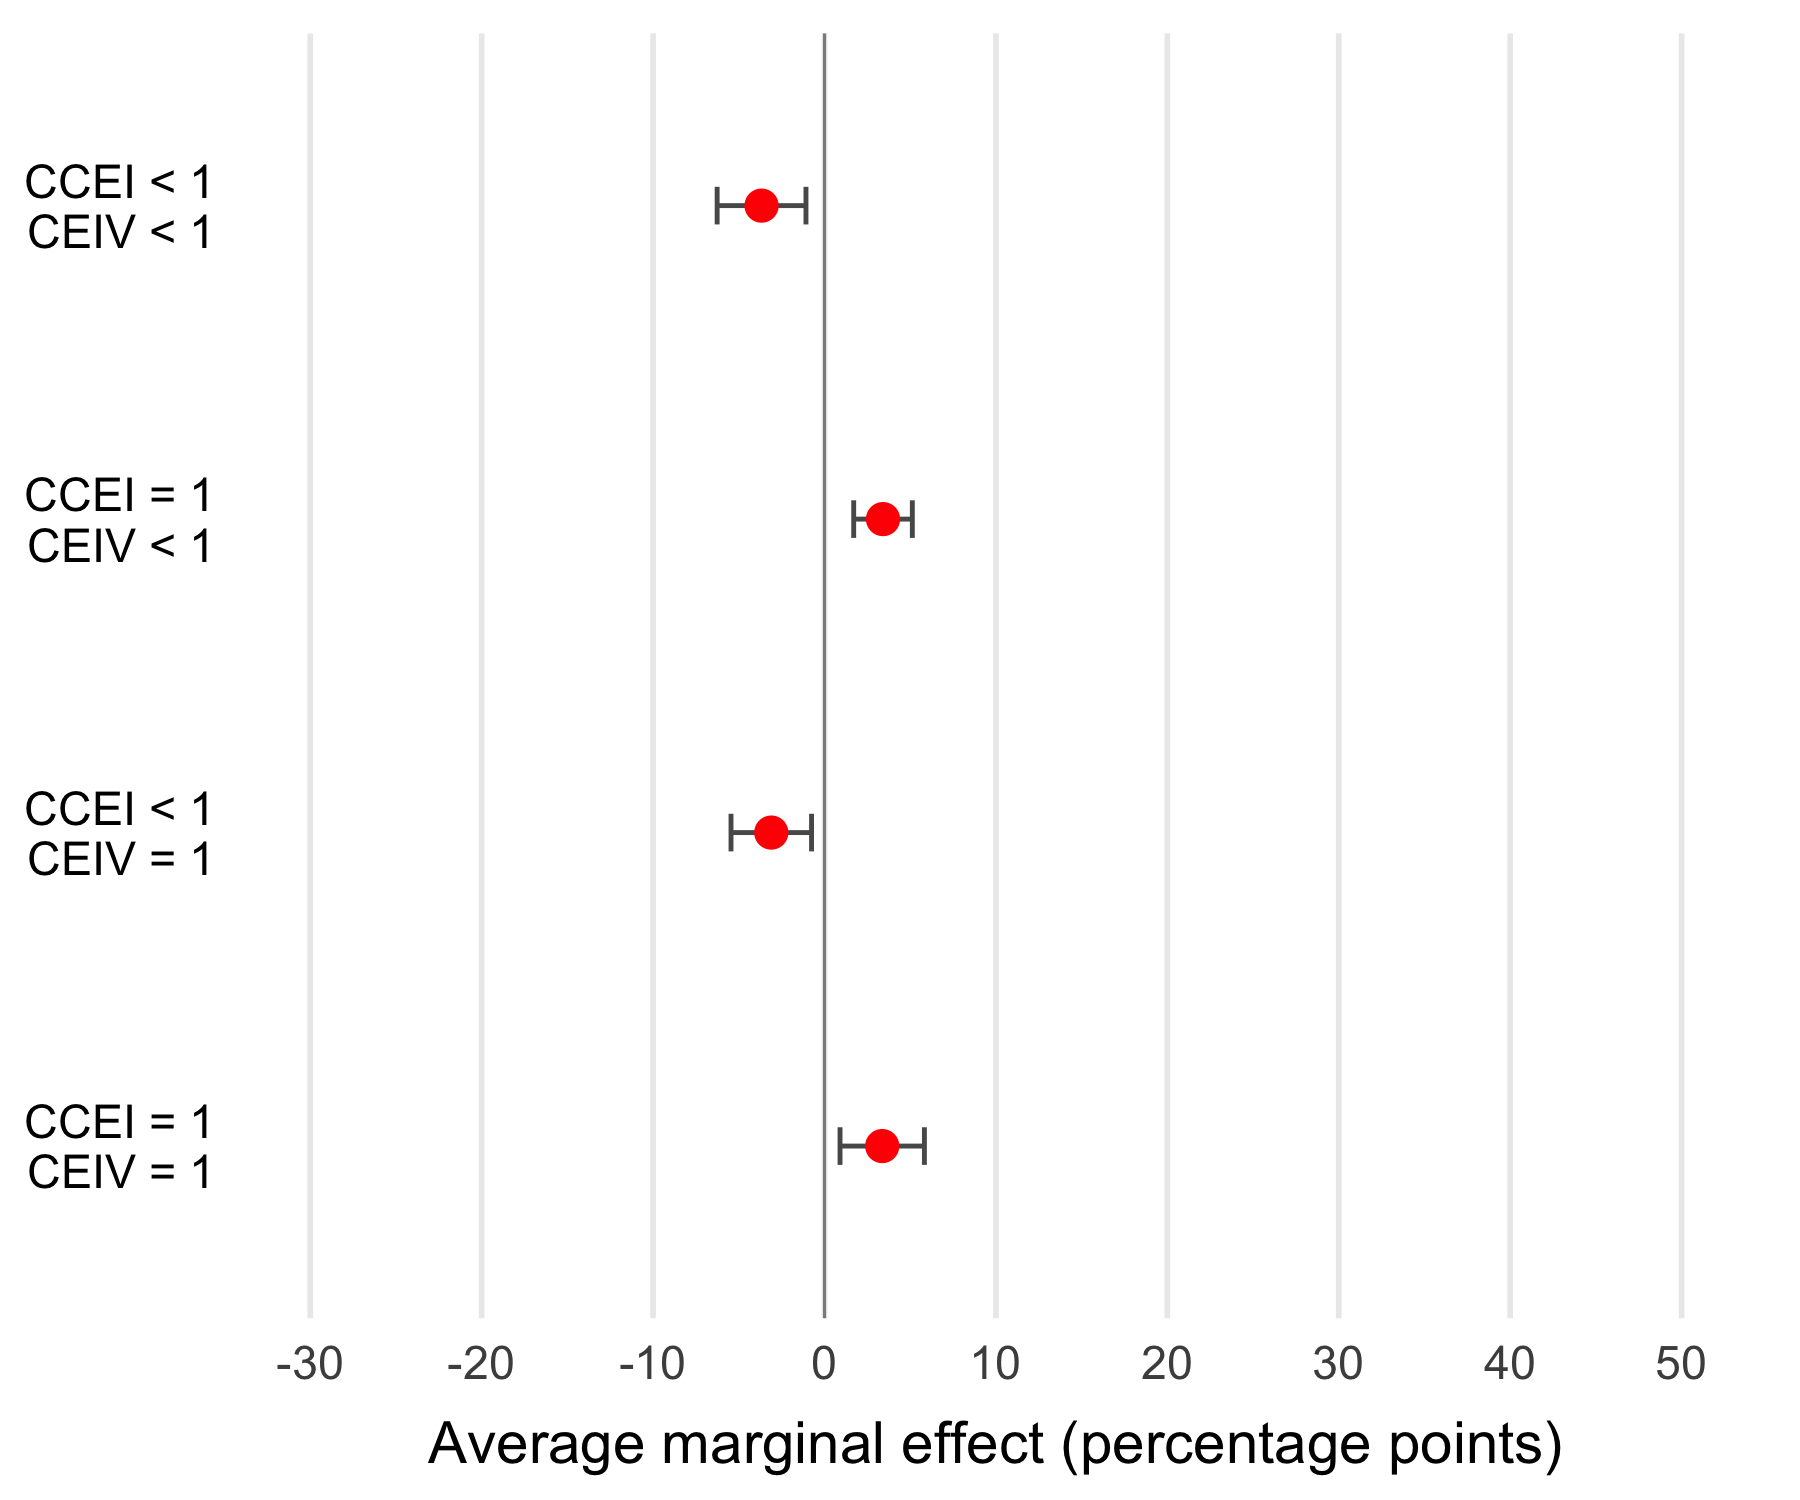
\includegraphics[width=\linewidth]{figure6_a_friend_0_ame_minimum.png}
\textbf{(b) Less rational member: minimum CCEI}\end{minipage}\end{center}
\begin{center}\begin{tabular}{lrrrr}\toprule
Outcome & CCEI $<1$, CEIV $<1$ & CCEI $=1$, CEIV $<1$ & CCEI $<1$, CEIV $=1$ & CCEI $=1$, CEIV $=1$\\\midrule
Observed pair-waves & 306 & 80 & 206 & 320\\
Share & 33.6\% & 8.8\% & 22.6\% & 35.1\%\\\bottomrule\end{tabular}\end{center}
\footnotesize\textit{Notes:} Effects are percentage points per 0.1 increase in individual CCEI, holding the other member's CCEI and controls fixed locally, then averaging over this subgroup. Four-category effects sum to zero for each member. Intervals use class-clustered standard errors. The class effects, coefficients, and outcome distributions can differ across separate fits; visual comparisons are descriptive.
\clearpage
\begin{center}\Large\textbf{One-sided friendship nomination}\end{center}
\small Directed friendship nominations distinguish none, one-sided, and mutual. Eligible counts are 912/225/167 pair-waves. The no-nomination figure duplicates the corresponding binary-friendship reference.
Separate-subgroup fit: 225 pair-waves, 185 distinct pairs, 58 class clusters.
\begin{center}\begin{minipage}{0.48\textwidth}\centering
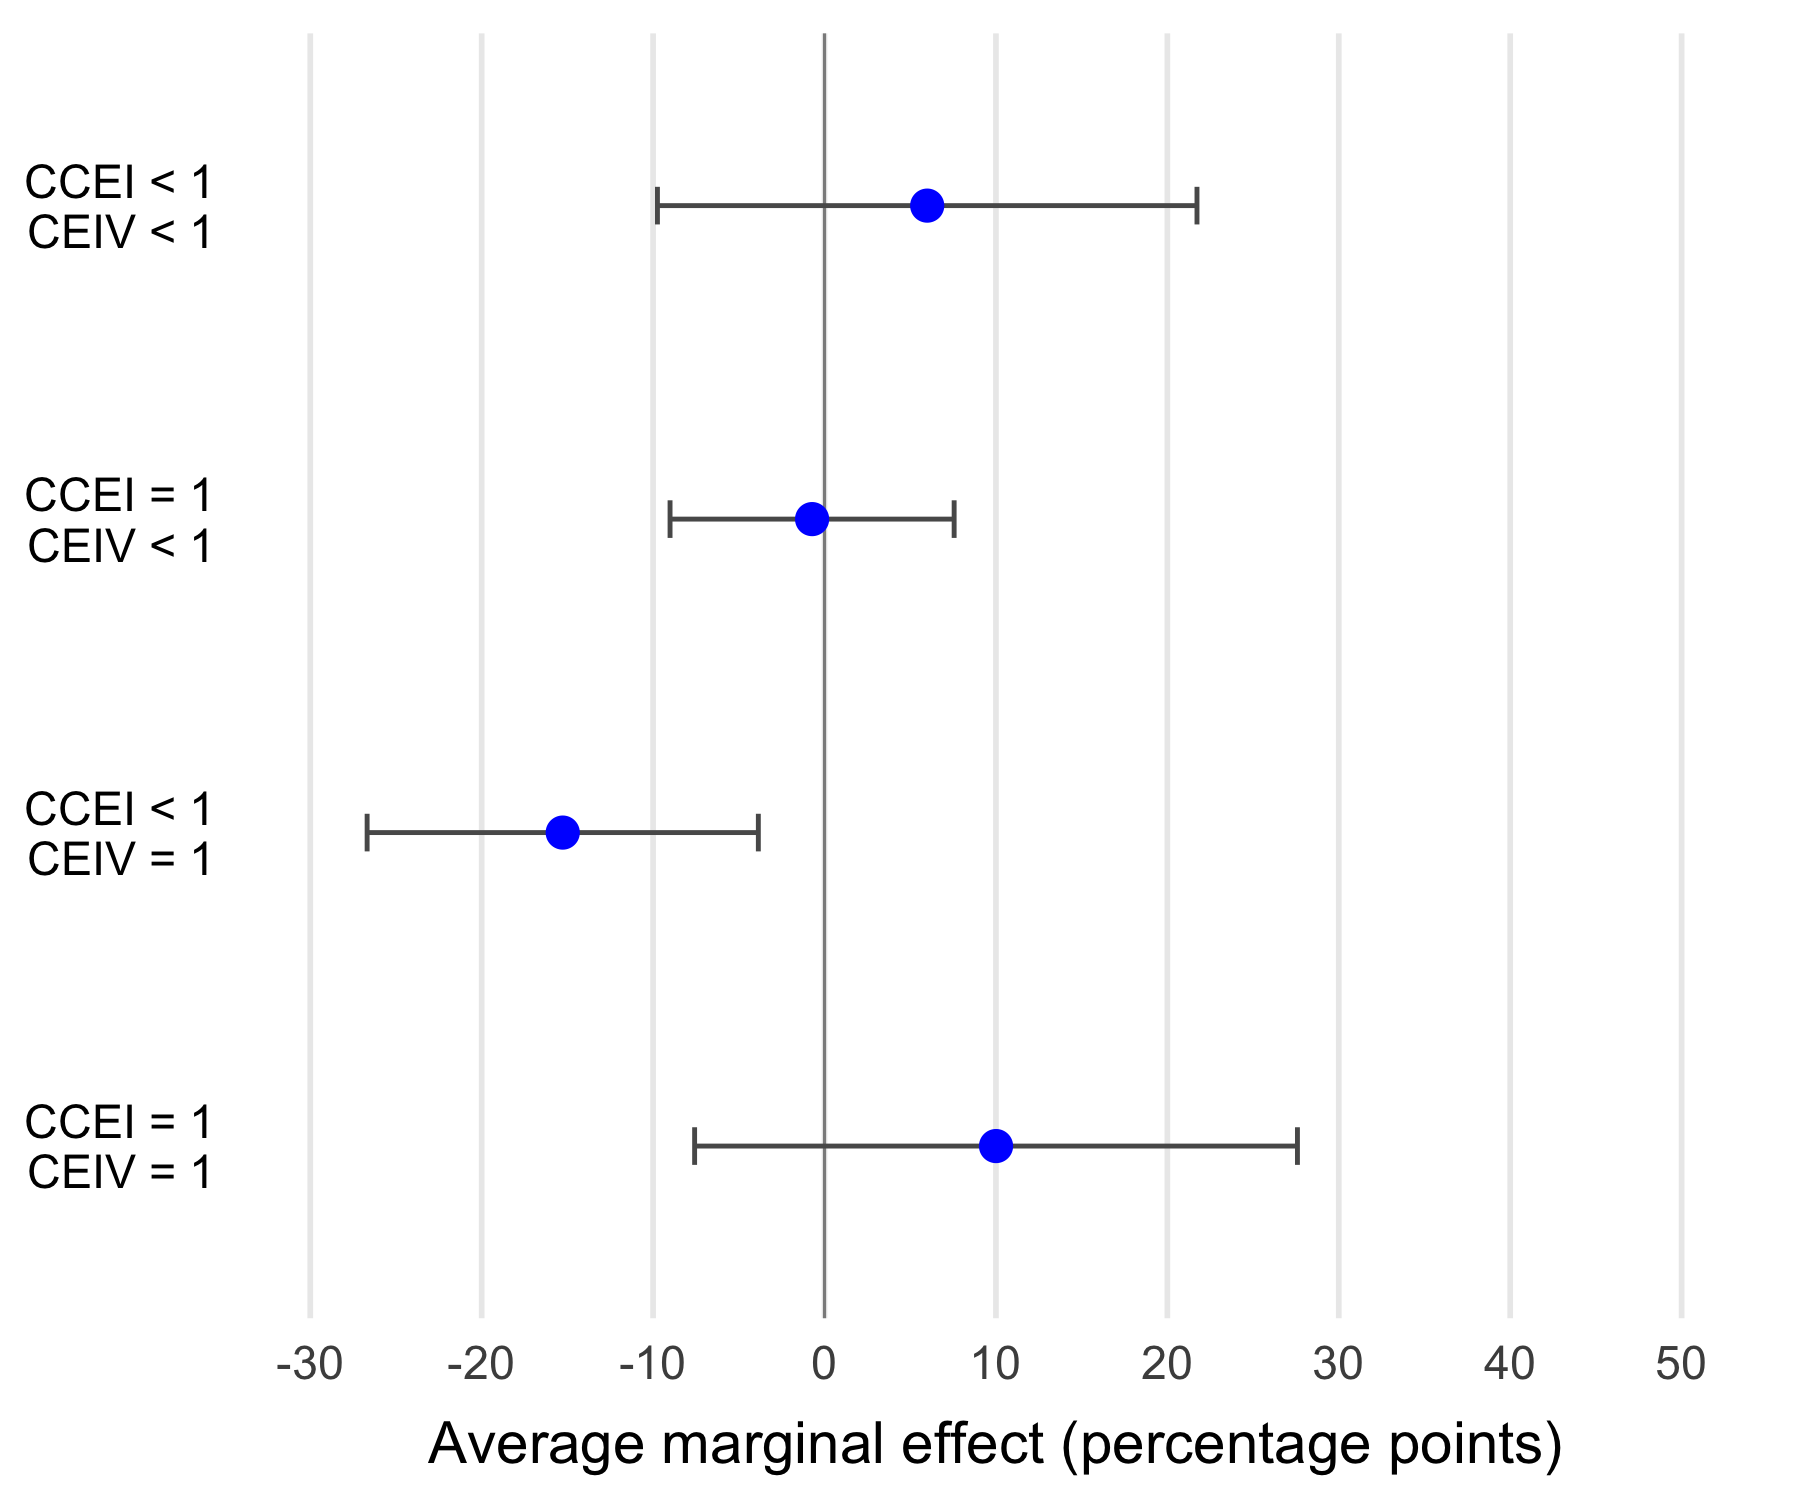
\includegraphics[width=\linewidth]{figure6_a_friend_1_ame_maximum.png}
\textbf{(a) More rational member: maximum CCEI}\end{minipage}\hfill\begin{minipage}{0.48\textwidth}\centering
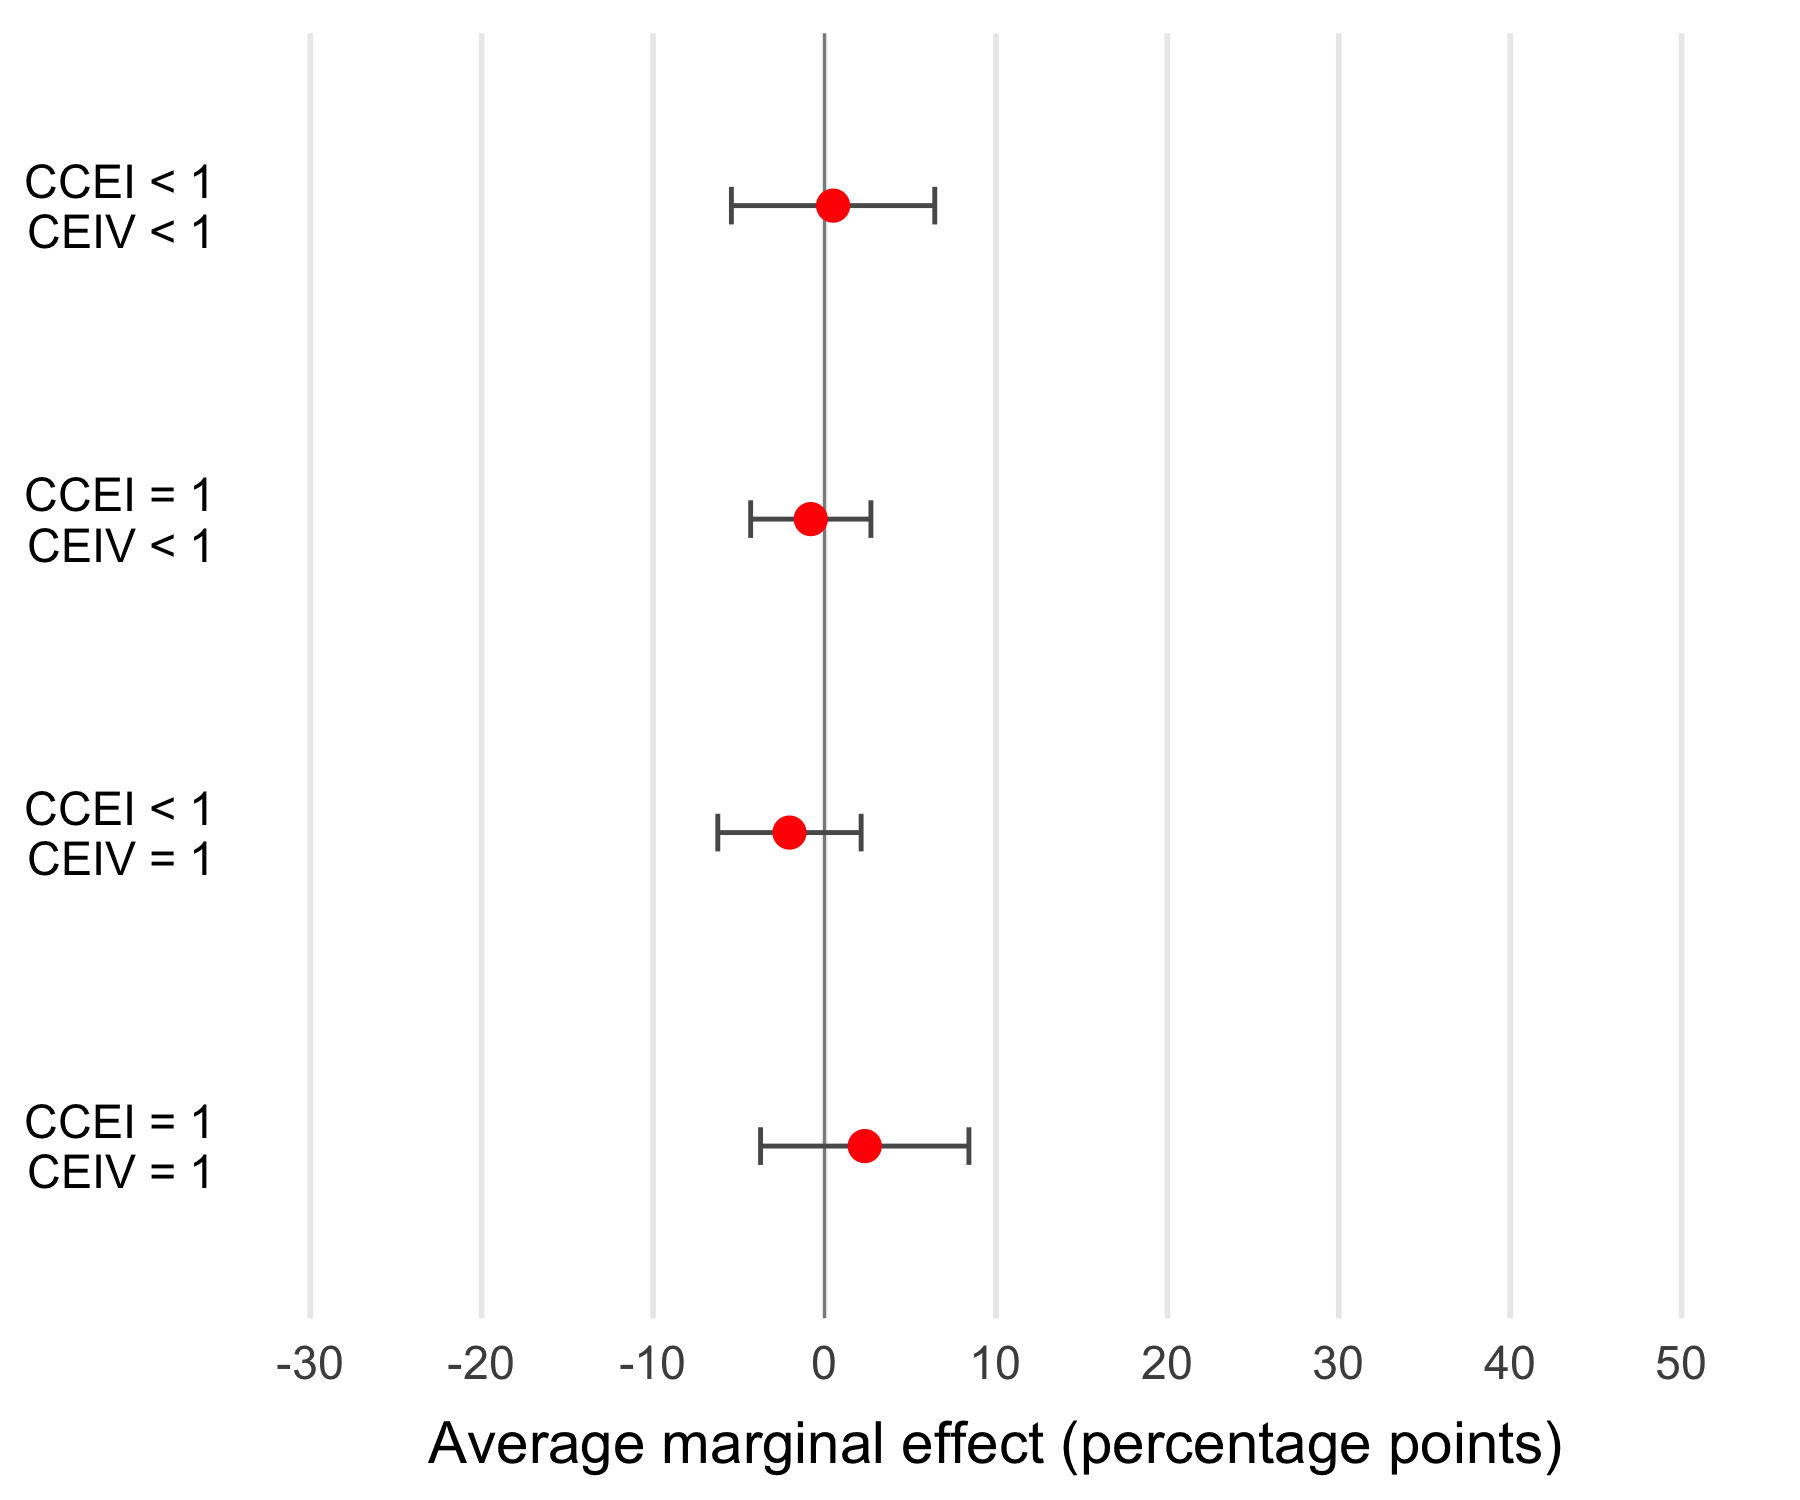
\includegraphics[width=\linewidth]{figure6_a_friend_1_ame_minimum.png}
\textbf{(b) Less rational member: minimum CCEI}\end{minipage}\end{center}
\begin{center}\begin{tabular}{lrrrr}\toprule
Outcome & CCEI $<1$, CEIV $<1$ & CCEI $=1$, CEIV $<1$ & CCEI $<1$, CEIV $=1$ & CCEI $=1$, CEIV $=1$\\\midrule
Observed pair-waves & 60 & 17 & 49 & 99\\
Share & 26.7\% & 7.6\% & 21.8\% & 44.0\%\\\bottomrule\end{tabular}\end{center}
\footnotesize\textit{Notes:} Effects are percentage points per 0.1 increase in individual CCEI, holding the other member's CCEI and controls fixed locally, then averaging over this subgroup. Four-category effects sum to zero for each member. Intervals use class-clustered standard errors. The class effects, coefficients, and outcome distributions can differ across separate fits; visual comparisons are descriptive.
\clearpage
\begin{center}\Large\textbf{Mutual friendship nomination}\end{center}
\textcolor{red!65!black}{\textbf{Shared-controls alternative; not an exact separate-subgroup replication.}}
\small Directed friendship nominations distinguish none, one-sided, and mutual. Eligible counts are 912/225/167 pair-waves. The no-nomination figure duplicates the corresponding binary-friendship reference.
The model fits all 1,304 pair-waves (64 class clusters), allowing friendship-specific slopes for both individual CCEIs. Marginal effects are averaged over the 167 mutual-friendship observations only. Other controls and class effects are shared across friendship categories.
\begin{center}\begin{minipage}{0.48\textwidth}\centering
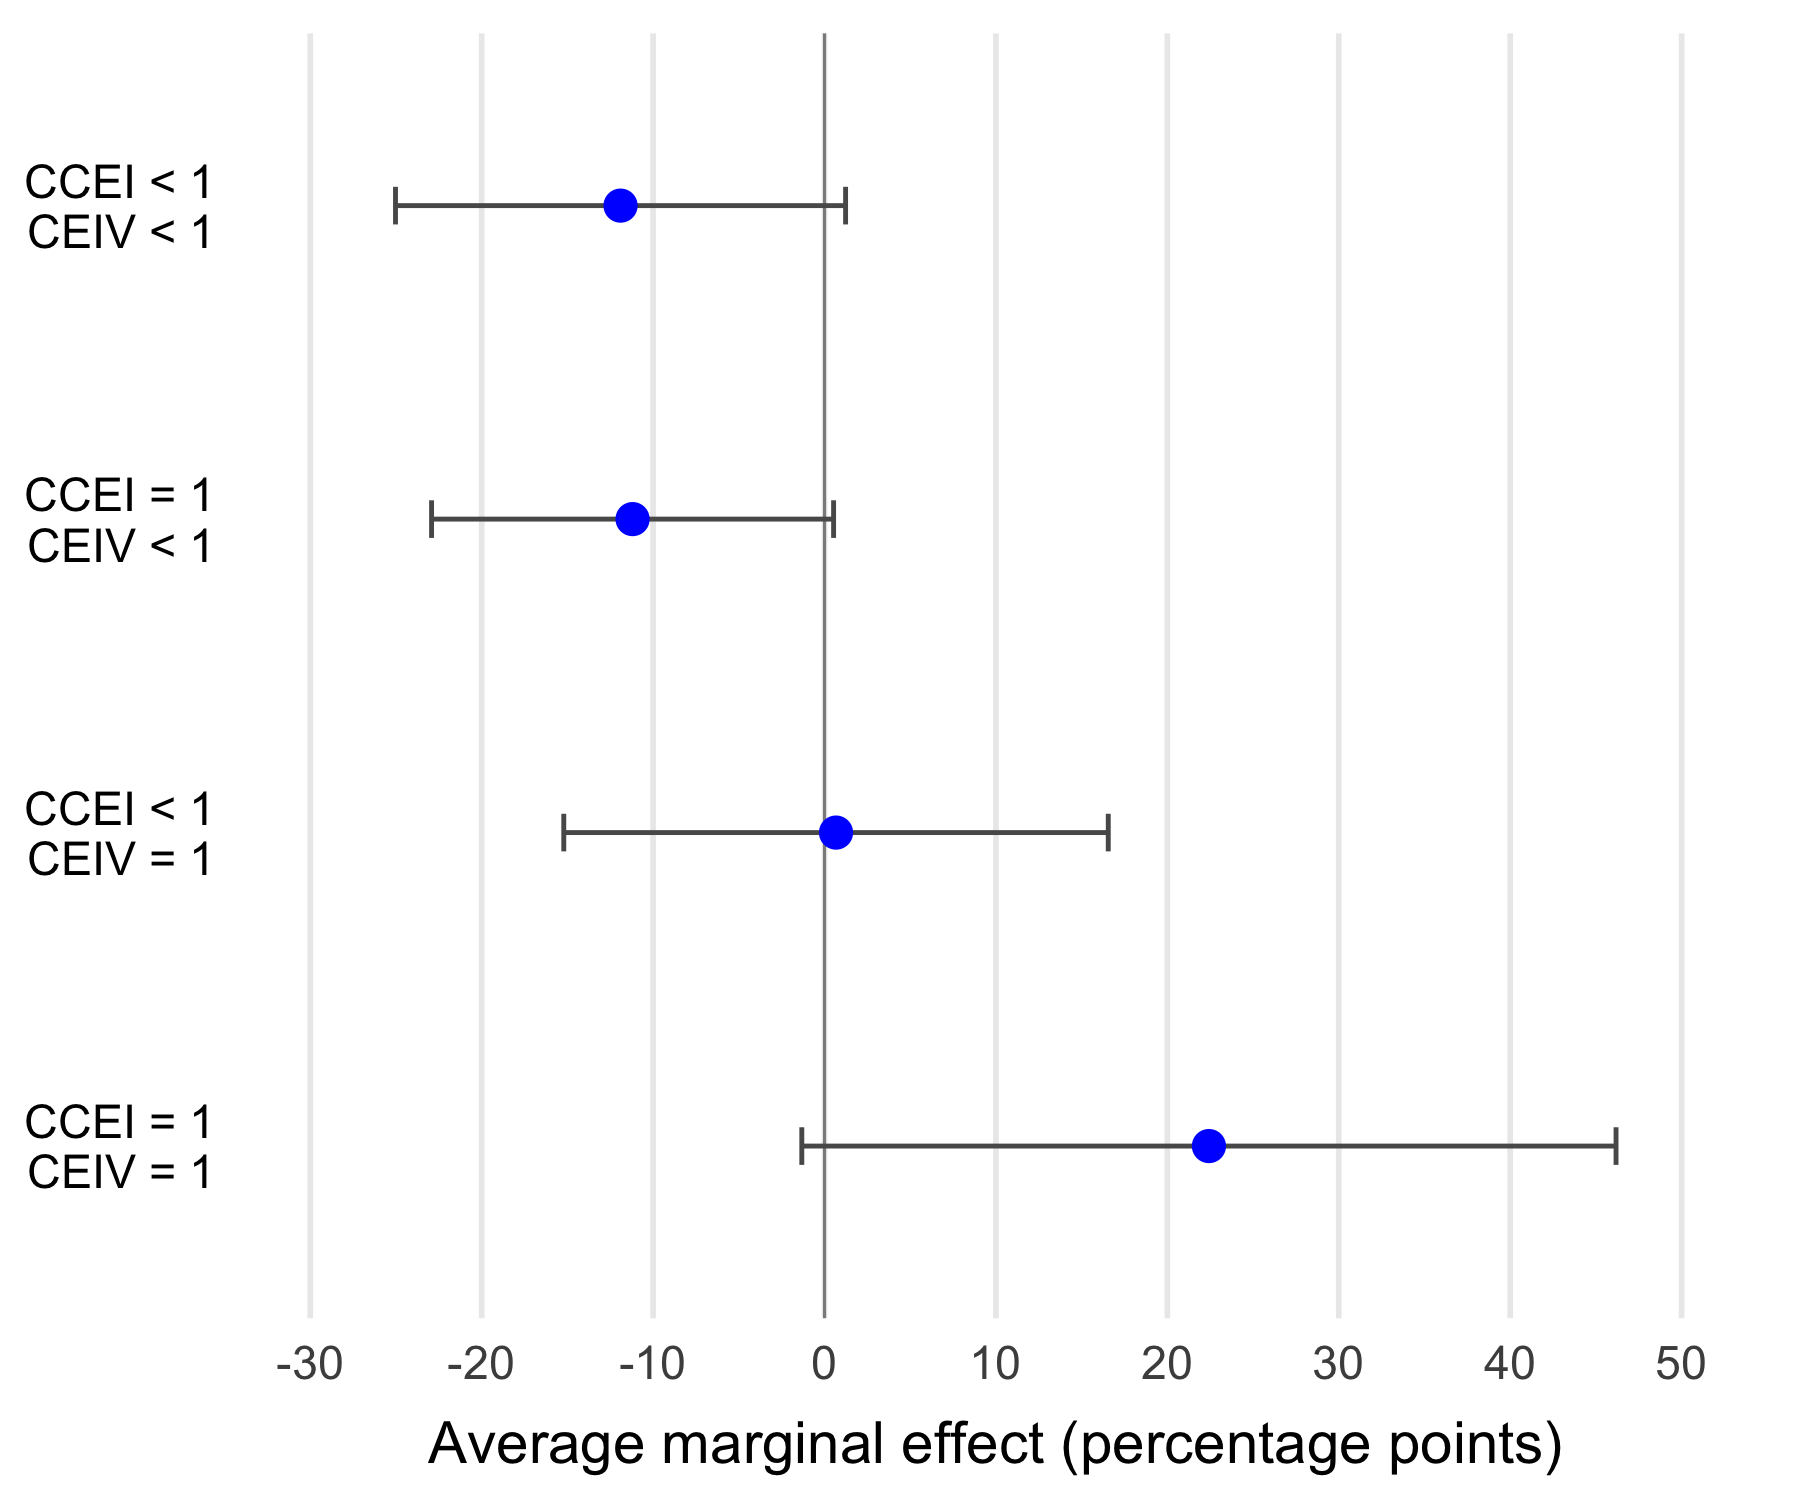
\includegraphics[width=\linewidth]{figure6_a_friend_pool_2_ame_maximum.png}
\textbf{(a) More rational member: maximum CCEI}\end{minipage}\hfill\begin{minipage}{0.48\textwidth}\centering
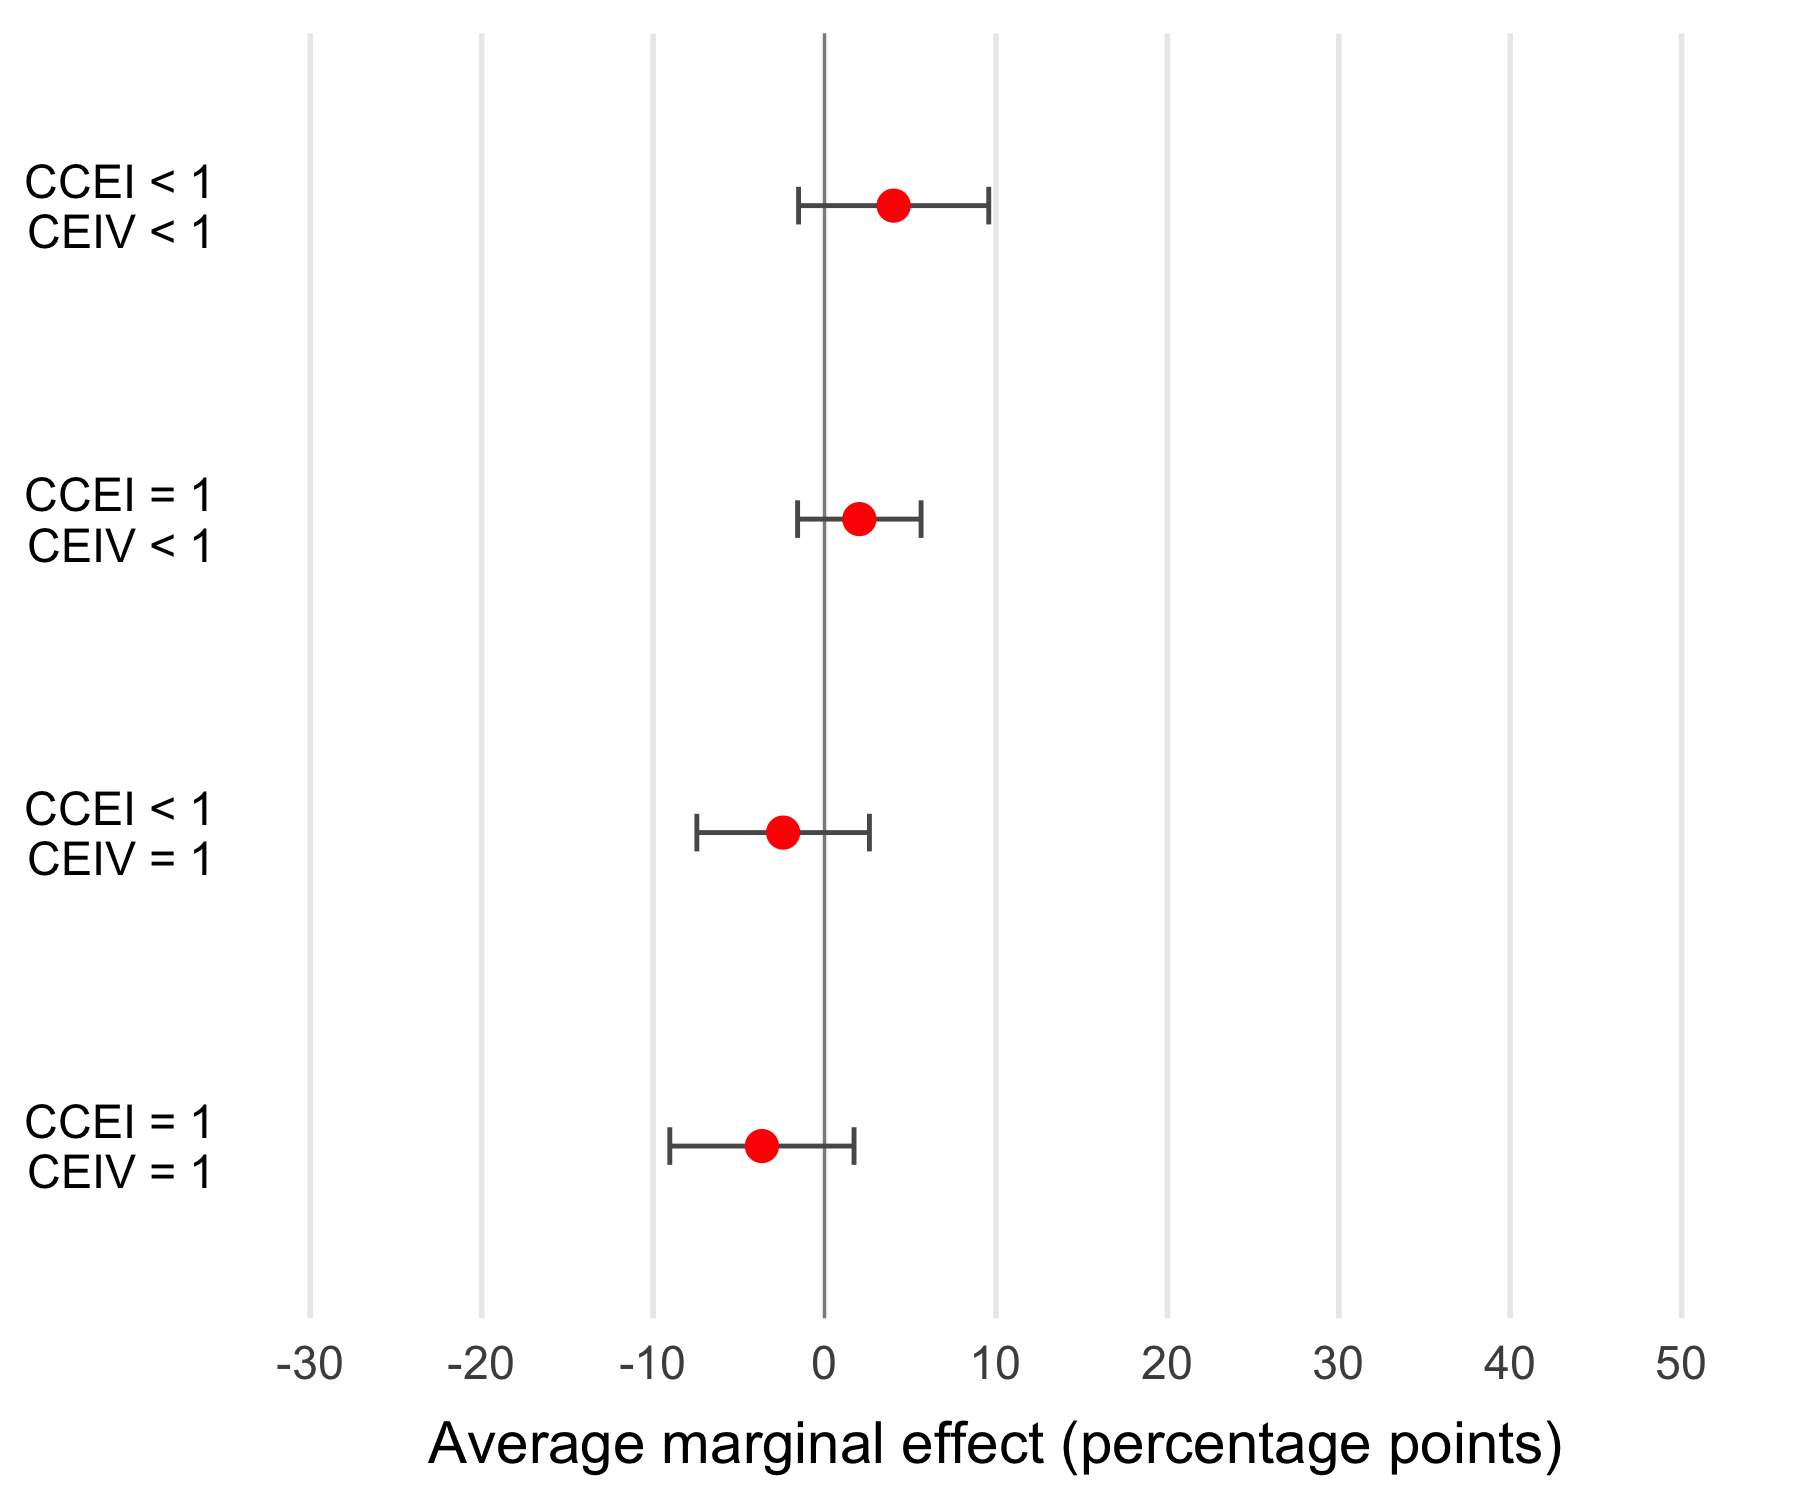
\includegraphics[width=\linewidth]{figure6_a_friend_pool_2_ame_minimum.png}
\textbf{(b) Less rational member: minimum CCEI}\end{minipage}\end{center}
\begin{center}\begin{tabular}{lrrrr}\toprule
Outcome & CCEI $<1$, CEIV $<1$ & CCEI $=1$, CEIV $<1$ & CCEI $<1$, CEIV $=1$ & CCEI $=1$, CEIV $=1$\\\midrule
Observed pair-waves & 49 & 20 & 45 & 53\\
Share & 29.3\% & 12.0\% & 26.9\% & 31.7\%\\\bottomrule\end{tabular}\end{center}
\footnotesize\textit{Notes:} Effects are percentage points per 0.1 increase in individual CCEI, holding the other member's CCEI and controls fixed locally, then averaging over this subgroup. Four-category effects sum to zero for each member. Intervals use class-clustered standard errors. The class effects, coefficients, and outcome distributions can differ across separate fits; visual comparisons are descriptive.
The exact separate mutual-friendship fit did not converge; the exported status table records this failure. The shared-controls results depend on the pooling restriction and serve as a sensitivity check.
\end{document}
